\documentclass[hyperref={pdfpagelabels=false}]{beamer}
\usepackage{helvet}
\usepackage[english]{babel}
\usepackage{pgfplots}
\usepackage{pgf}
\pgfplotsset{compat=newest}
\usepackage{booktabs}
\usepackage[T1]{fontenc}
\usepackage[utf8]{inputenc}
\usepackage{lipsum}
\usepackage{tcolorbox}
\usepackage{xcolor}
\usepackage{listings}
\usepackage[nopatch=footnote]{microtype}
\usepackage{float}
\usepackage{siunitx}
\usepackage{multicol}
\usepackage{hyperref}
\usepackage{dsfont}
\usepackage{caption}
\usepackage{subcaption}
\usepackage[backend=biber,style=authoryear-comp,sorting=nyt]{biblatex} % Package for bibliography (citing)
\bibliography{bibliography.bib}
\graphicspath{{./img}}

% DTU colours for diagrams
% You might want to make the front/back page background colour the first colour in the plot cycle list.
\pgfplotscreateplotcyclelist{DTU}{%
dtured,         fill=dtured,        \\%
blue,           fill=blue,          \\%
brightgreen,    fill=brightgreen    \\%
navyblue,       fill=navyblue       \\%
yellow,         fill=yellow         \\%
orange,         fill=orange         \\%
grey,           fill=grey           \\%
red,            fill=red            \\%
green,          fill=green          \\%
purple,         fill=purple         \\%
}

% Table of contents (TOC) and numbering of headings
\setcounter{tocdepth}{1}    % Depth of table of content: sub sections will not be included in table of contents
\setcounter{secnumdepth}{2} % Depth of section numbering: sub sub sections are not numbered



\newcommand{\setcolor}[1]{\def\chosencolor{#1}}
\newcommand{\setdepartment}[1]{\def\department{#1}}

\setbeamerfont{caption}{size=\tiny}

% \setbeamersize{text margin left=22mm}

\usetikzlibrary{shapes, shapes.callouts, positioning, arrows.meta, calc}
\usepackage{eurosym}
\usepackage{animate}

%%% Local Variables:
%%% mode: LaTeX
%%% TeX-master: "main"
%%% End:

% \includeonlyframes{current}
\title{Reverse ADL-Vickrey}
\subtitle{Inferring Scheduling Preferences based on Congestion and Choice Data}
\author{Pietro Giardina}

\begin{document}


\section{Introduction} % Vickrey
\begin{frame}
  \tableofcontents[currentsection]
\end{frame}

\begin{frame}
  \frametitle{Is Congestion a Problem?}
  According to a recent study\footcite{kim2022congestion},
  \begin{itemize}
  \item An \textbf{average} delay of 4-5 minutes \textbf{per commuter} is caused by congestion
  \item This damage is worth, in California, \textbf{1.67\%} of the state GDP.
  \end{itemize}
\end{frame}

\begin{frame}
  \frametitle{How is congestion created?}
  \begin{figure}
    \centering
    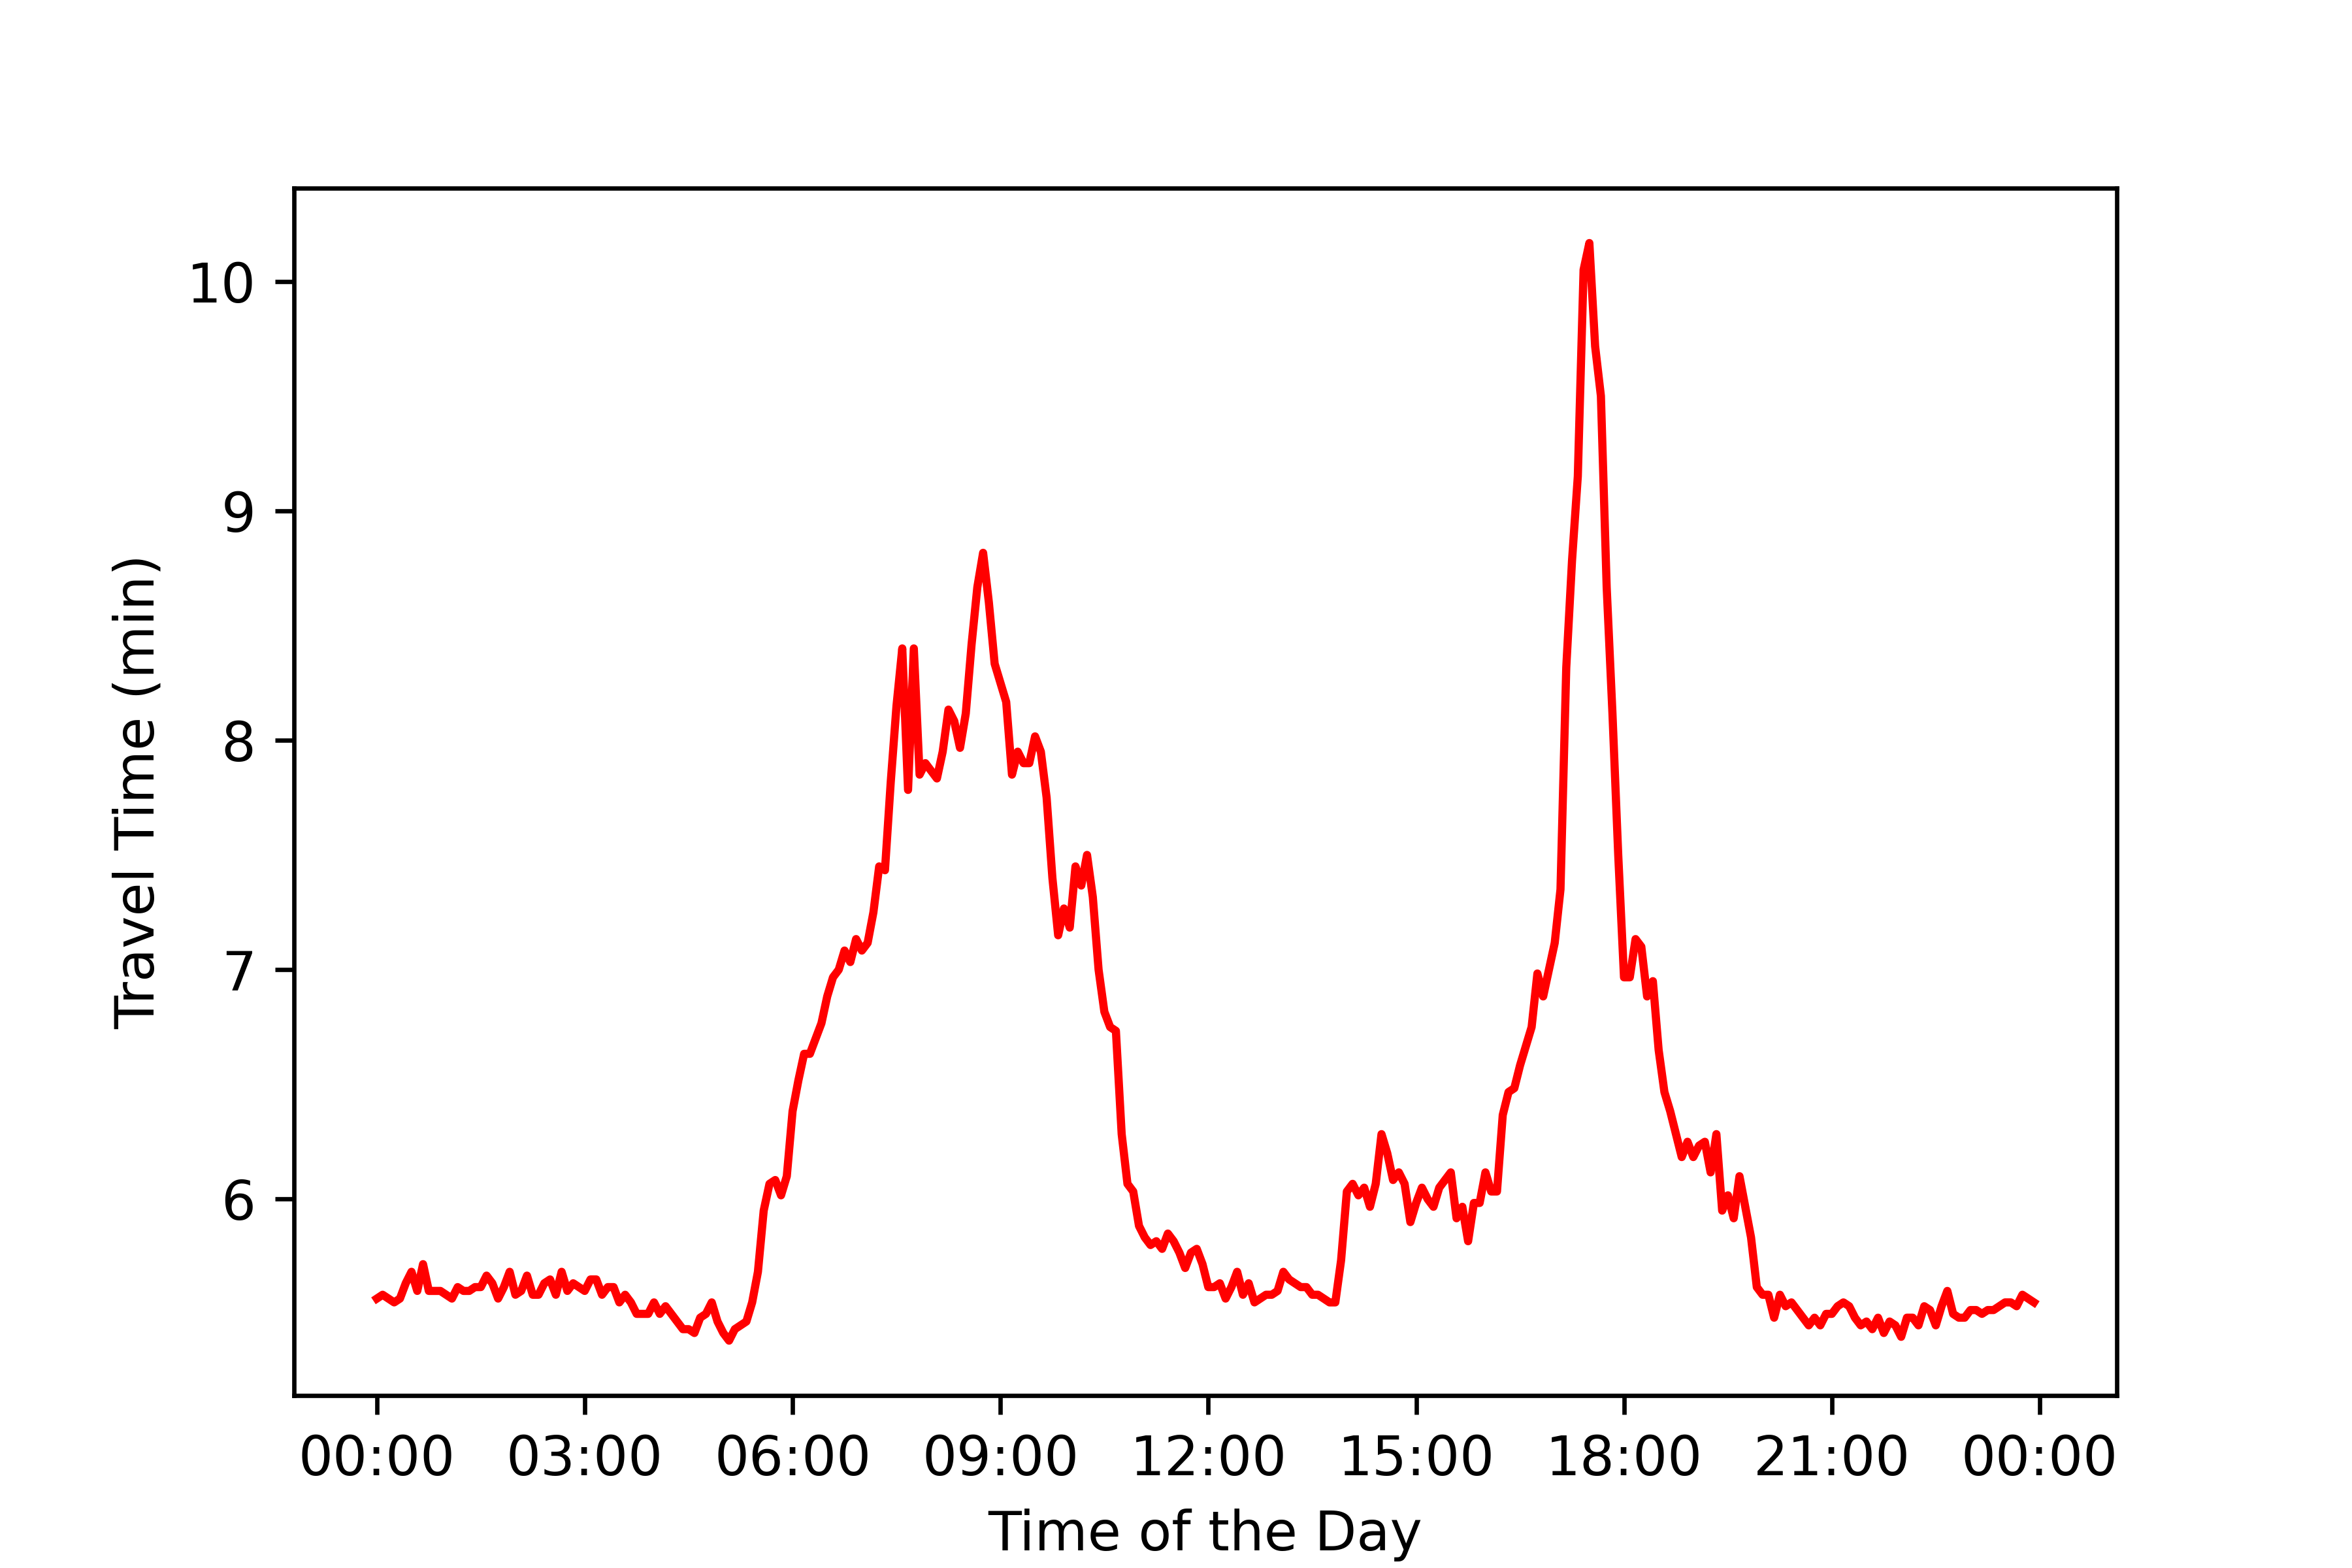
\includegraphics[width=.7\textwidth]{travel_time}
    \caption{Travel Time, on California State Route 237, the 16th of February 2018.
    Data from CalTrans PeMS.}
    \label{fig:tt}
  \end{figure}
  \begin{itemize}
  \item All commuters want to travel at the same time, with the same mode
  \item<2-> The infrastructure saturates beyond capacity
  \end{itemize}
\end{frame}

\begin{frame}
  \frametitle{How can congestion be tackled?}
  On demand side, Travel Demand Management:
  \begin{itemize}
  \item<2-> Influencing mode choice
  \item<3-> Influencing route/destination choice
  \item<4-> Incentivize spreading of departure times
  \end{itemize}

  \visible<4->{How can we have an impact on when people decide to leave?}
\end{frame}

\begin{frame}
  \frametitle{When do People Travel?}
  According to the bottleneck model\footcite{f32d6720-dd02-34b7-a4ba-c4c21193efe7, d0907f84-e14a-3d98-ad20-759f41491d6e},
  minimising three main discomforts:
  \begin{itemize}
  \item Travel time
  \item Arriving too early
  \item Arriving too late
  \end{itemize}

  \visible<2->{The cost is assumed to grow linearly on these three components}
\end{frame}

\begin{frame}
  \frametitle{The \(\alpha\)-\(\beta\)-\(\gamma\) Model}
  Each commuter minimizes a cost function (from \cite{d0907f84-e14a-3d98-ad20-759f41491d6e})
  \begin{equation*}
    C(t_d) = \alpha(\text{travel time}) + \beta (\text{time early}) + \gamma (\text{time late})
  \end{equation*}
  \begin{figure}
    \centering
    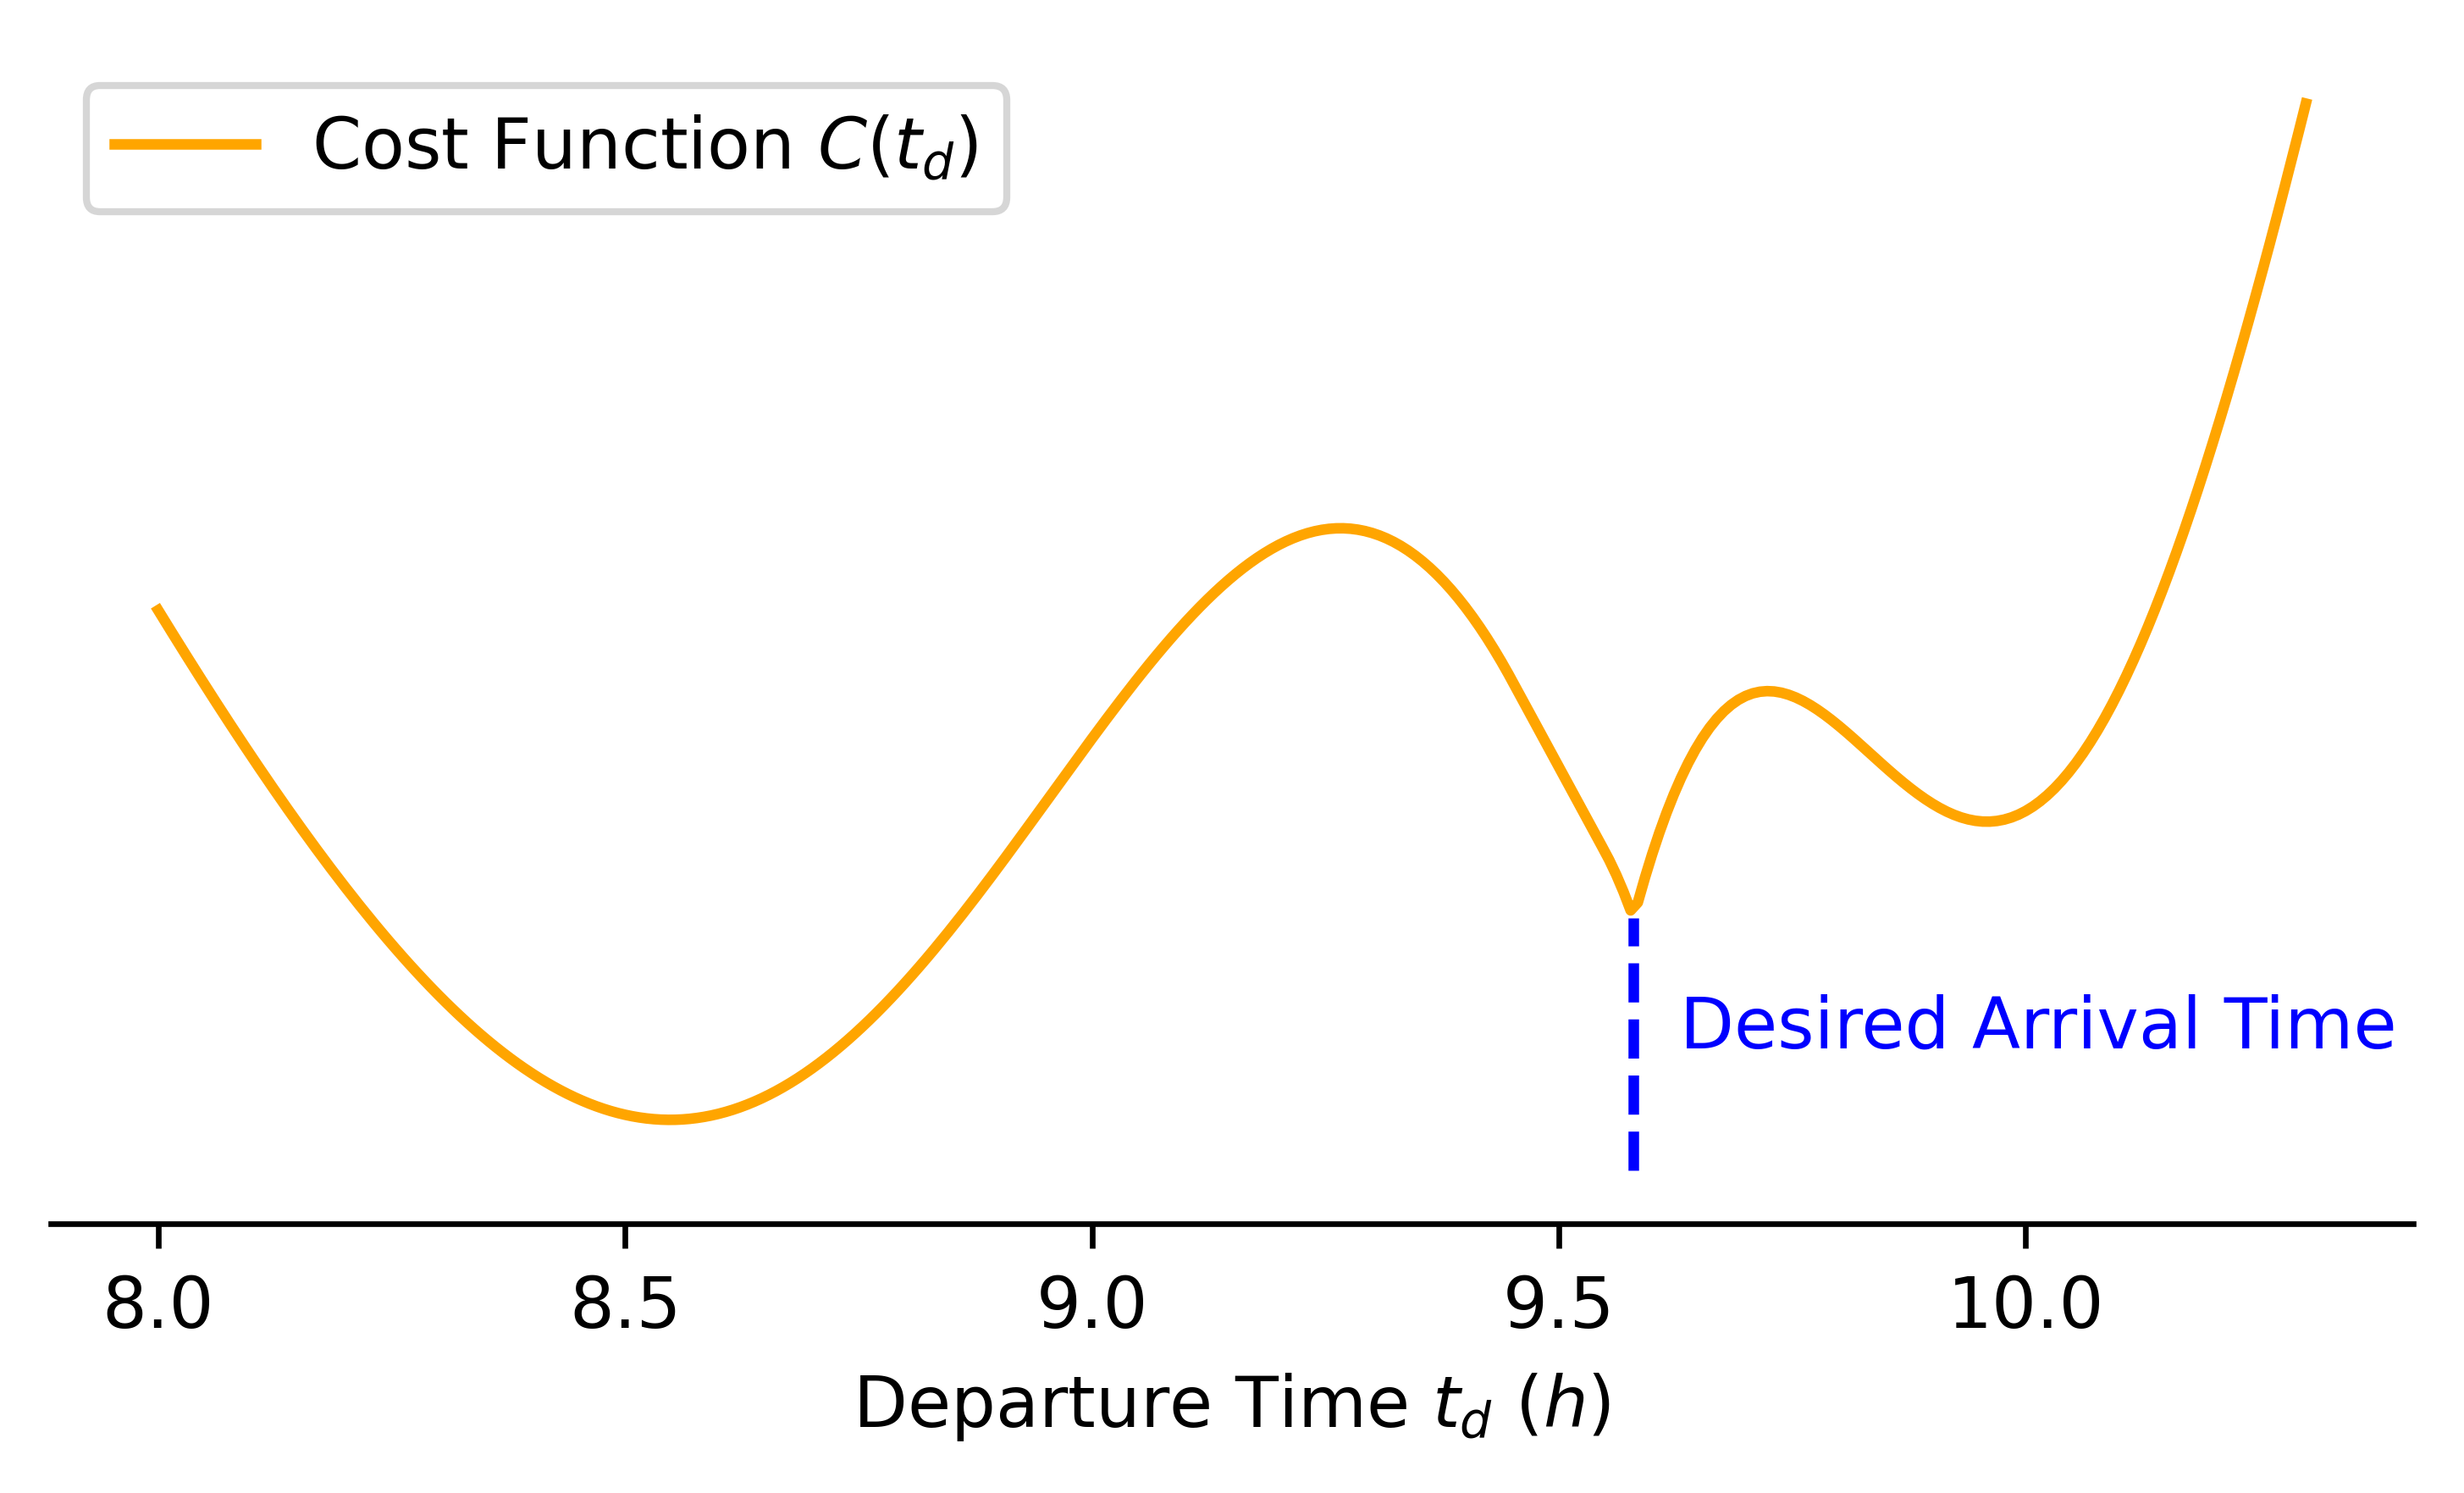
\includegraphics[width=.7\textwidth]{cost_simple}
  \end{figure}
\end{frame}

\begin{frame}
  \frametitle{Calibrating the Parameters}
  For many applications, it is important to find values for \(\alpha\), \(\beta\) and \(\gamma\) (\textit{scheduling preferences}).
  \begin{itemize}
  \item<2-> Historically, estimation was done with surveys
  \item<3-> \textcite{54d203ee-4bf8-3234-9286-56e4c8b7f5bd} estimates the following:
    \begin{equation*}
      \frac{\beta}{\alpha} = 0.61\qquad \frac{\gamma}{\alpha} = 2.38
    \end{equation*}
  \item<4-> \textcite{https://doi.org/10.1111/iere.12692} presents a brief review of the results
  \end{itemize}
\end{frame}

\begin{frame}
  \frametitle{Weaknesses of Surveys}
  Surveys are extremely costly, and can suffer from many sources of error
  \begin{itemize}
  \item<2-> Answers may be biased, due to reasons beyond the control of the scientist
  \item<3-> Rounding may limit the precision
  \end{itemize}

  
\begin{tikzpicture}[overlay, remember picture]
    \node[
    ellipse callout,
    callout relative pointer={(-1,-1)},
    fill=red!70,
    text width=5.5cm,
    align=center,
    above right,
    xshift=2cm,
    yshift=1.8cm
    ] (Q) at (current page.south west) {How much should I pay you for arriving 5 minutes earlier to work?};
    \node[
    ellipse callout,
    callout relative pointer={(.5,-.5)},
    fill=red!70,
    % text width=3cm,
    align=center,
    below right=.5cm of Q,
    xshift=1cm,
    % yshift=2cm
    ] (A) {\(x\) \euro};
  \end{tikzpicture}
\end{frame}
\begin{frame}
  \frametitle{Revealed Preferences data}
  Data about Revealed Preferences may offer some advantages
  \begin{itemize}
  \item<2-> A priori, more precise
  \item<3-> Can be systematically harvested
  \item<4-> More difficult to elaborate
  \end{itemize}
\end{frame}

\begin{frame}
  \frametitle{Research Question}
  Can we calibrate the parameters \(\alpha\), \(\beta\) and \(\gamma\) by using only Revealed Preferences?
\end{frame}

\section{Methodology}
\begin{frame}
  \tableofcontents[currentsection]
\end{frame}

\begin{frame}
  \frametitle{The Idea}
  From data that are objectively measurable,
  we estimate the values for scheduling preferences:
  
  \begin{figure}
    \centering
    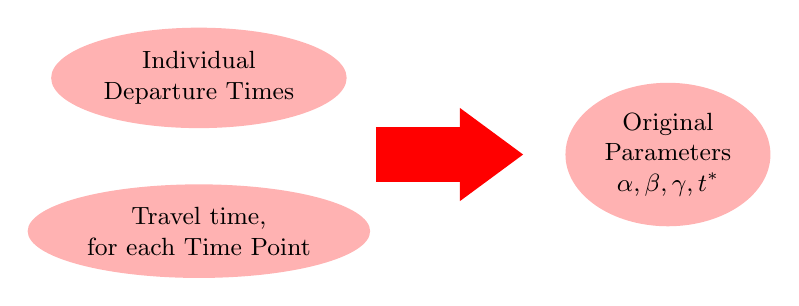
\begin{tikzpicture}
      \node[
      align=center,
      ellipse,
      fill=red!30,
      font=\small
      ] (dep) {Individual\\ Departure Times};
      \node[
      align=center,
      ellipse,
      fill=red!30,
      font=\small,
      below = .7 cm of dep
      ] (tt) {Travel time,\\for each Time Point};
      \node[right = 2cm of {$(dep) !.5! (tt)$}] (mid) {};
      \draw[
      -{Triangle[width=32pt,length=23pt]},
      line width=20pt,
      red
      ] (mid) -- ++(2.0cm,0);
      \node[
      right=2.4 cm of mid,
      align=center,
      ellipse,
      fill=red!30,
      font=\small,
      ] {Original\\Parameters \\\(\alpha, \beta, \gamma, t^*\)};
    \end{tikzpicture}
  \end{figure}
\end{frame}

\begin{frame}
  \frametitle{Working Principle}
  The development of the model is done in three main steps:
  \begin{enumerate}
  \item<2-> The optimal departure time is theoretically studied
  \item<3-> A function, expressing the likelihood of a data point, is found
  \item<4-> Maximising the likelihood, the parameters are estimated
  \end{enumerate}
\end{frame}

\begin{frame}
  \frametitle{Evaluation of the Model}
  Progressively more complex evaluations are possible:
  \begin{enumerate}
  \item<2-> Evaluation on a Synthetic Dataset
  \item<2-> Evaluation of data from a Traffic Simulator
  \item<2-> Evaluation on Real Data
  \end{enumerate}
\end{frame}

\section{Development of the Model}

\begin{frame}
  \tableofcontents[currentsection]
\end{frame}

\begin{frame}
  \frametitle{The Cost Function}
  \begin{figure}
    \centering
    % \animategraphics[palindrome, autoplay,controls={play, stop},width=.7\textwidth]{20}{animation_no_shades/frame_}{0}{79}
    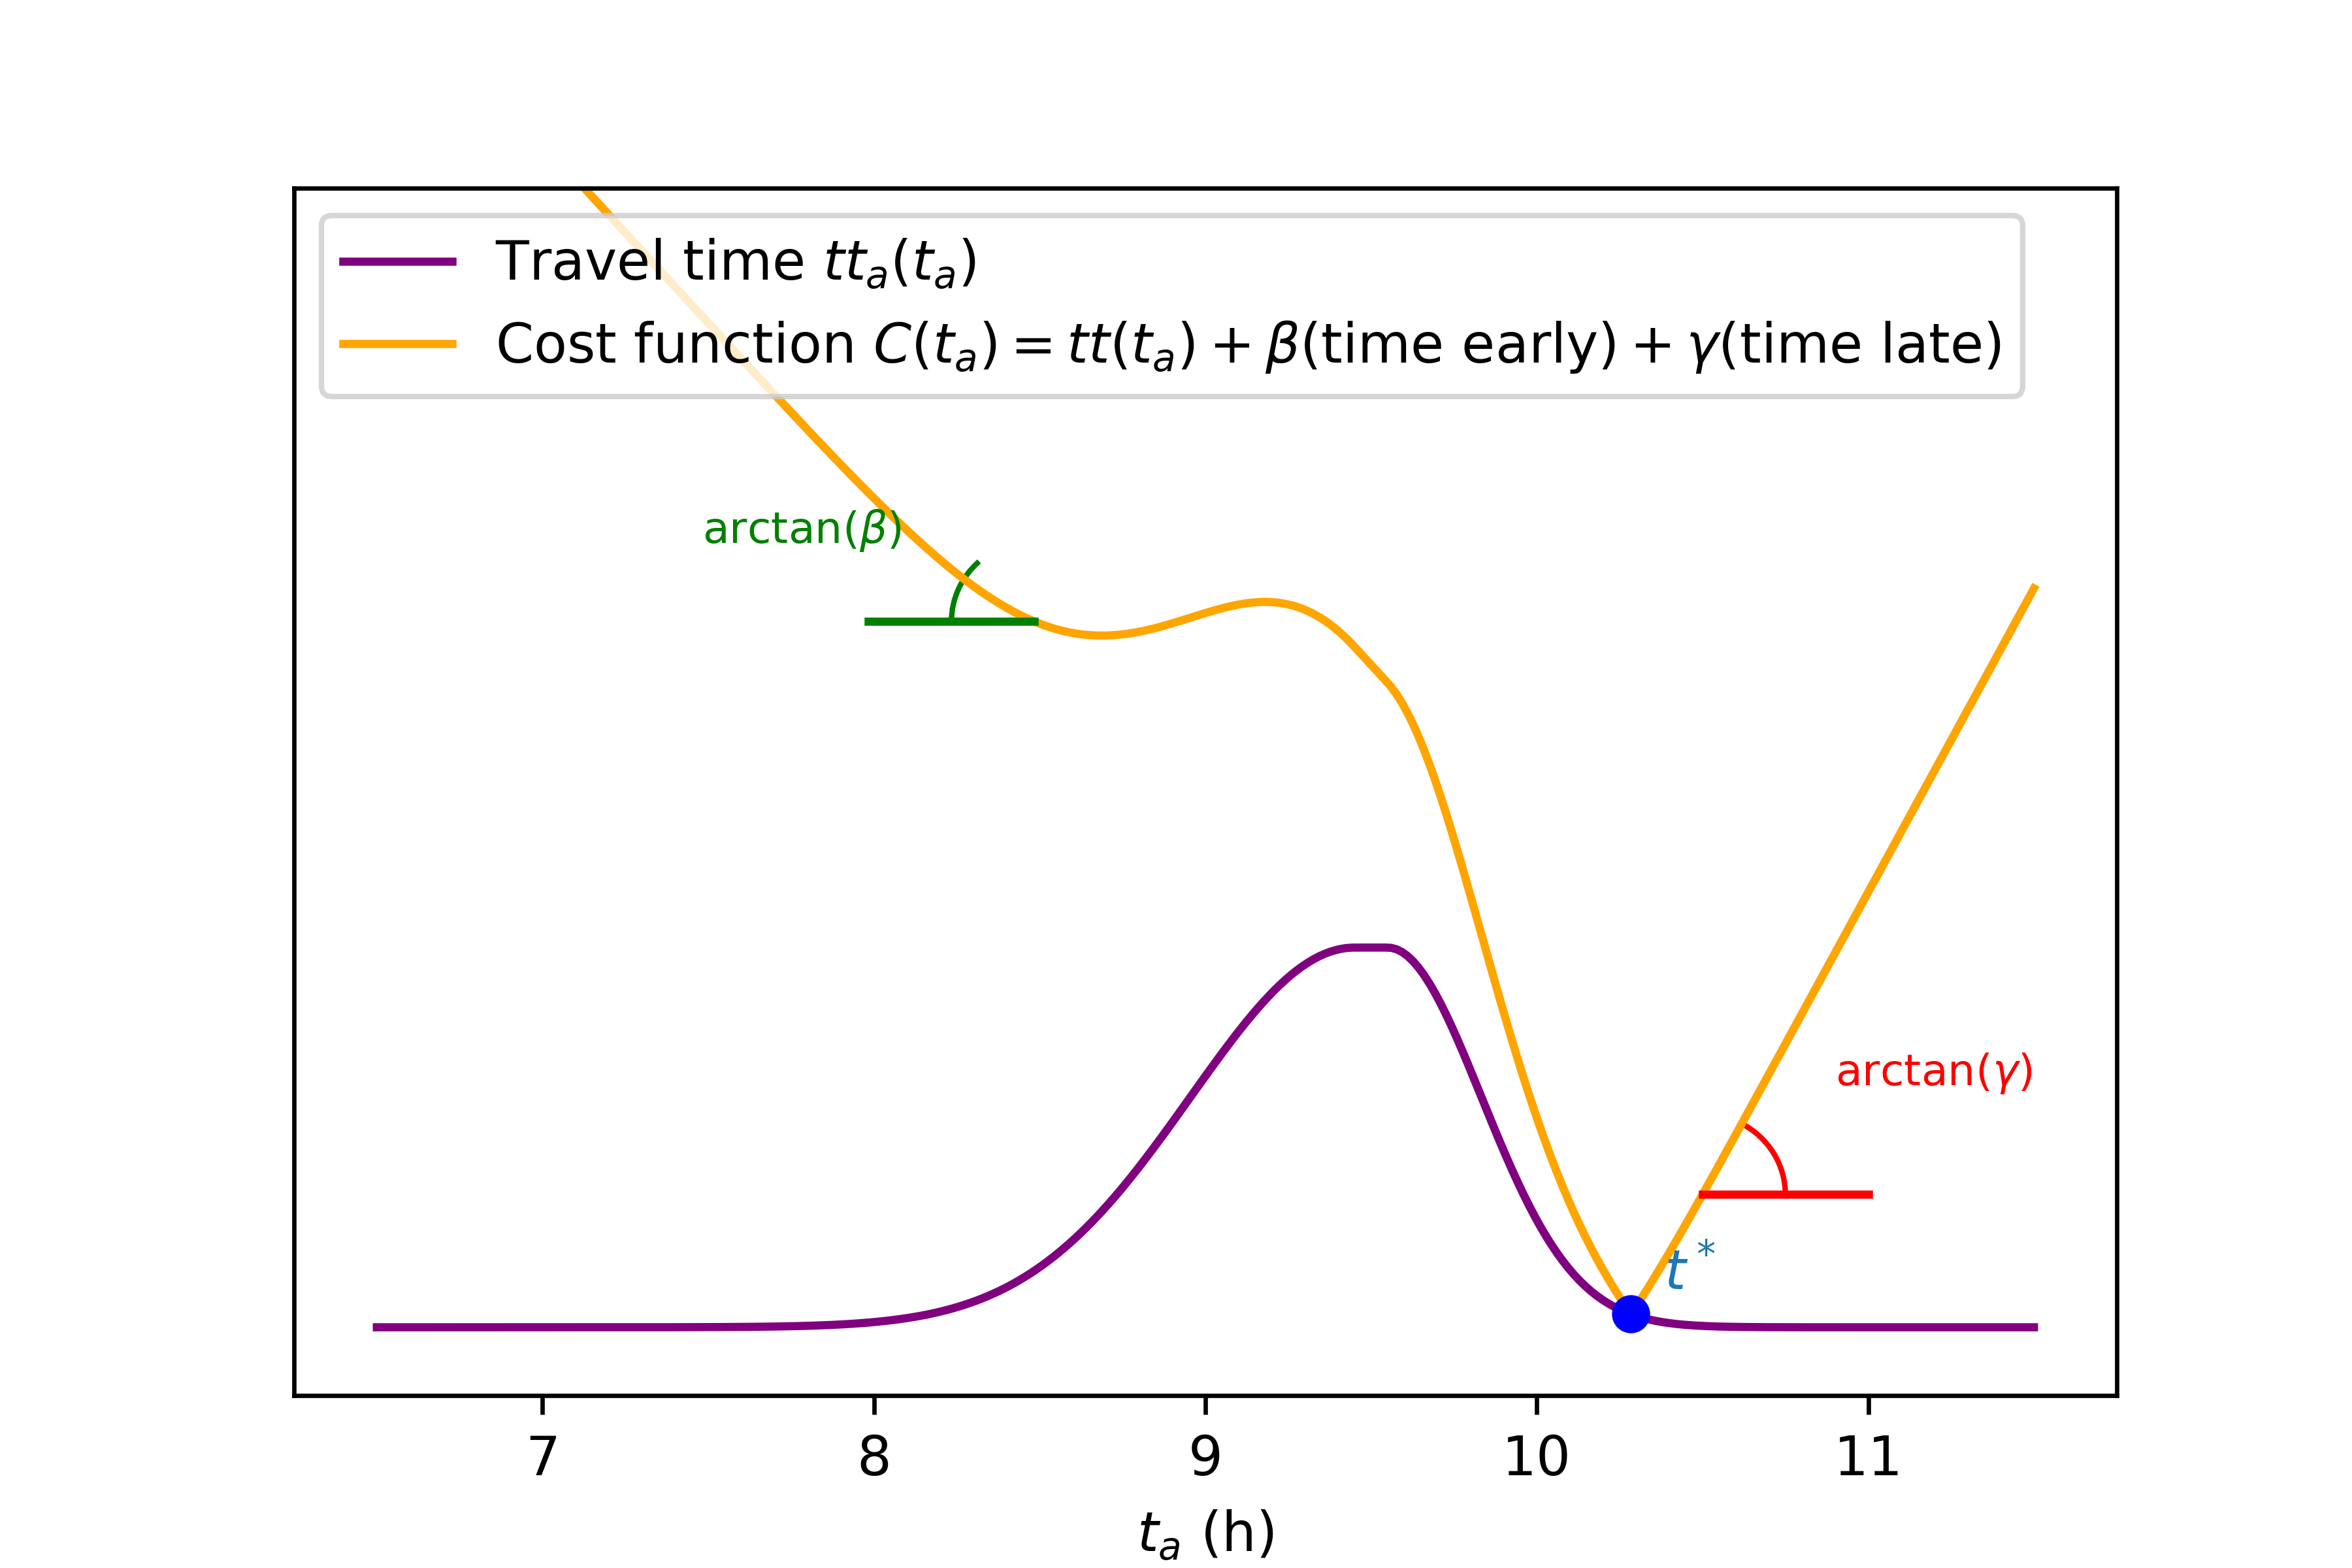
\includegraphics[width=.7\textwidth]{animation_no_shades/frame_79}
  \end{figure}
  Three different types of minima:
  \begin{itemize}
  \item \textcolor{green}{Early minima}
  \item \textcolor{blue}{On-time minima}
  \item \textcolor{red}{Late minima}
  \end{itemize}
\end{frame}

\begin{frame}
  \frametitle{Characterization of minima}
  Location of minima depends on tangents to the travel time function, given \(\alpha, \beta\) and \(\gamma\):
  \begin{figure}
    \centering
    % \animategraphics[palindrome, controls={play, stop},width=.8\textwidth]{20}{animation_shades/frame_}{0}{79}
    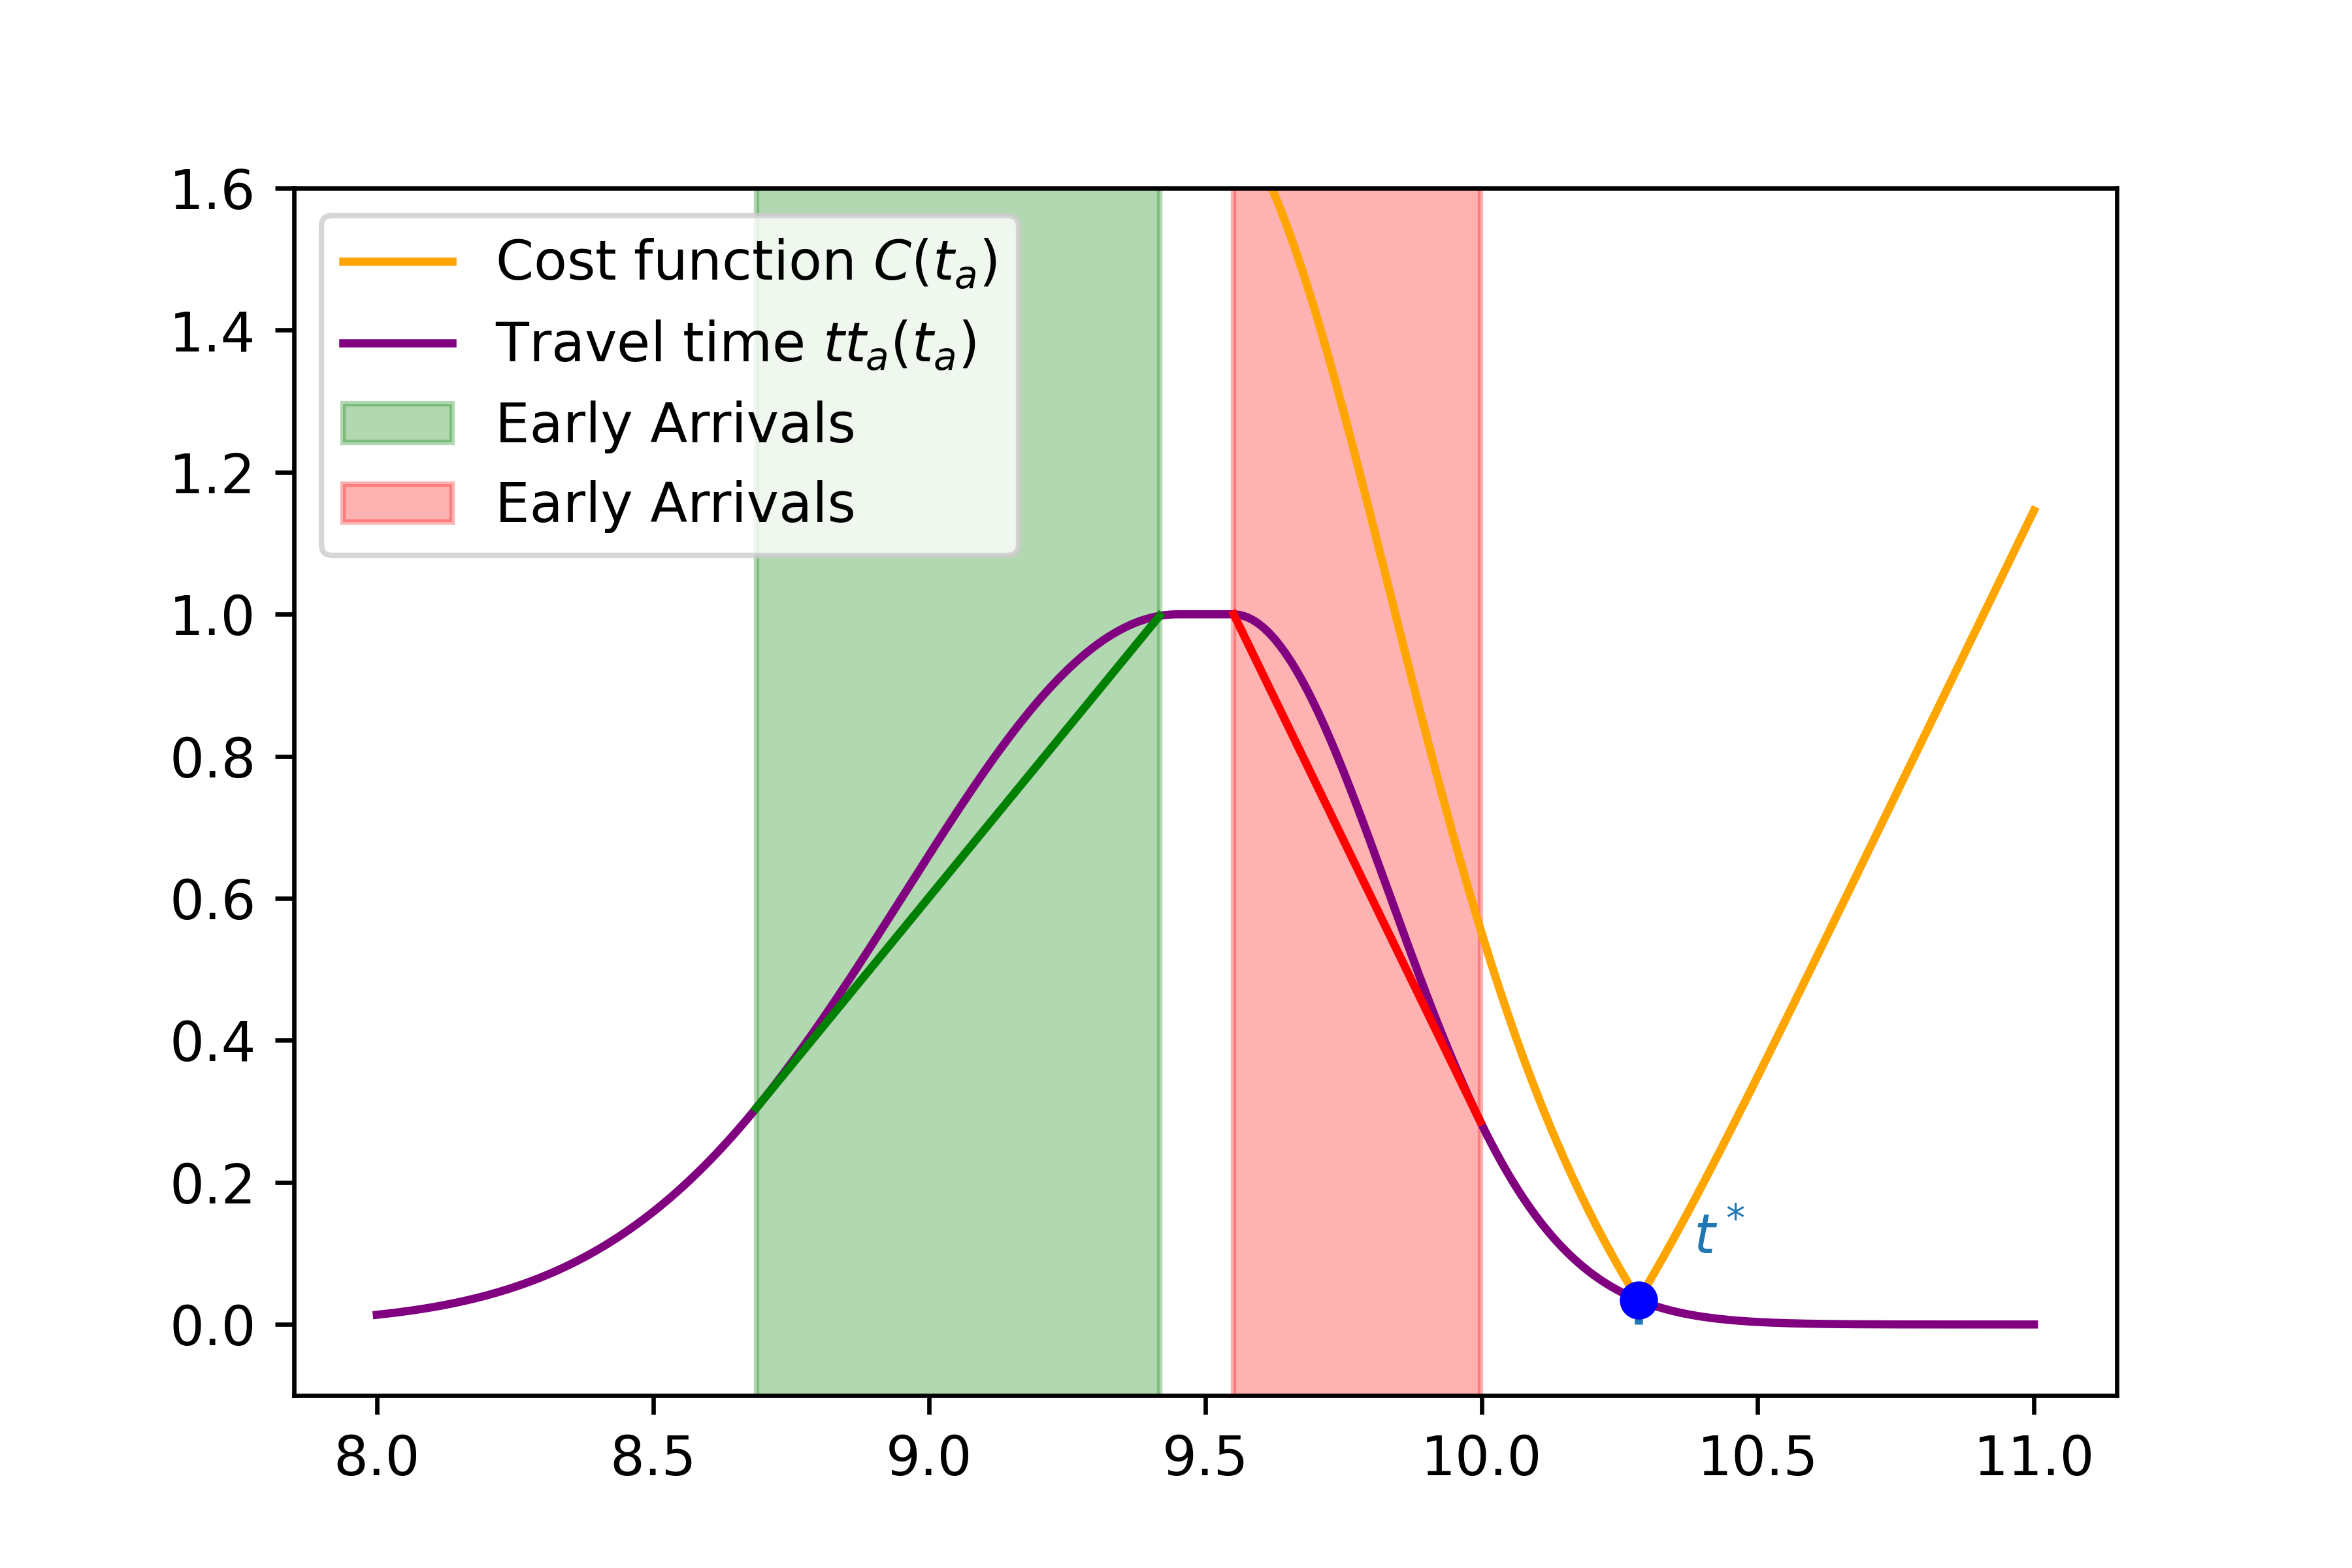
\includegraphics[width=.8\textwidth]{animation_shades/frame_79}
  \end{figure}
\end{frame}

\begin{frame}
  \frametitle{Computation of Likelihood}
  \begin{itemize}
  \item Given the characterization, an expression for the likelihood can be found:
  \scalebox{0.62}{\parbox{.5\linewidth}{
        \begin{align*}
          f_{T_a}(t_a) =
          & \color<2->{blue} f_{T^*}(t_a)\int_{\beta_0(t_a)}^{\beta_\text{max}}f_\beta(b)\, db\int_{\gamma_0(t_a)}^{\gamma_\text{max}}f_\gamma(g)\, dg \\
          & \color<2->{green}+ f_\beta(tt_a'(t_a))[tt_a''(t_a)]^+\int_1^\infty f_\gamma(x) \left(F_{T^*}(\min(b_e(tt_a'(t_a)), t_s(tt_a'(t_a), x))) - F_{T^*}(t_a)\right) dx\  \\
          & \color<2->{red}+ f_\gamma(tt_a'(t_a))[tt_a''(t_a)]^+  \int_0^1f_\beta(x) \left(F_{T^*}(t_a) - F_{T^*}(\max(g_i(-tt_a'(t_a)), t_s(x, -tt_a'(t_a)))) \right) dx\
        \end{align*}
      }}
  \item<2-> The expression for the likelihood is a sum of three different terms
    \begin{itemize}
    \item<2-> A term for \textcolor{blue}{on-time arrivals}
    \item<2-> A term for \textcolor{green}{early arrivals}
    \item<2-> A term for \textcolor{red}{late arrivals}
    \end{itemize}
  \end{itemize}
\end{frame}

\begin{frame}
  \frametitle{Maximising the Likelihood}
  By using the expression for the likelihood,
  scheduling delay parameters can be estimated:
  \begin{itemize}
  \item<2-> \(\beta, \gamma, t^*\) are assumed to be distributed
  \item<2-> The distributions are parametrized by a parameter \(\theta\)
  \item<3-> The likelihood yields a function \(\mathcal{L} : \theta \mapsto f_{T_a}(t_a | \theta)\)
  \item<4-> Maximising the likelihood, an estimate \(\hat{\theta}\) is found
  \end{itemize}
\end{frame}

\section{Evaluation of the Model}

\begin{frame}
  \tableofcontents[currentsection]
\end{frame}

\begin{frame}
  \frametitle{Evaluation on Synthetic Data}
  Evaluation is performed on a dataset built accordingly to the bottleneck model
  \begin{itemize}
  \item A value for the parameter \(\theta\) is chosen
  \item<2-> \(N\) samples are drawn from the distributions of \(\beta, \gamma, t^*\)
  \item<3-> For each of the \(N\) triple of samples, the cost function is minimized
  \item<4-> The model is run on the resulting dataset, yielding an estimate \(\hat{\theta}\) of the parameter \(\theta\)
  \end{itemize}
\end{frame}

\begin{frame}
  \frametitle{Choosing the Parameter $\theta$}
  Suppose the user characteristics distributed as
  \begin{equation*}
    \beta \sim \mathcal{N}(\mu_\beta, \sigma) \quad \gamma \sim \mathcal{N}(\mu_\gamma, \sigma) \quad t^* \sim \mathcal{N}(\mu_t, \sigma_t)
  \end{equation*}
  \visible<2->{\(\theta \in \mathbb{R}^5\) can be, for instance, chosen as follows:
  \begin{equation*}
    \theta = \begin{pmatrix}
      \mu_\beta \\
      \mu_\gamma \\
      \mu_t \\
      \sigma \\
      \sigma_t
    \end{pmatrix}
    =
    \begin{pmatrix}
      0.5 \\
      1.4 \\
      9.5 \\
      0.3 \\
      1
    \end{pmatrix}
  \end{equation*}}
\end{frame}

\begin{frame}
  \frametitle{Sampling Arrival Times}
  Arrival times are found by minimizing the cost.
  \begin{itemize}
  \item Independently minimizing the cost for \(N = 100,000\) samples, the following distribution is found
  \item<2-> The theoretical likelihood, for the original value of \(\theta\), closely resembles the empirical distribution
  \end{itemize}
  \centering
  \alt<1>{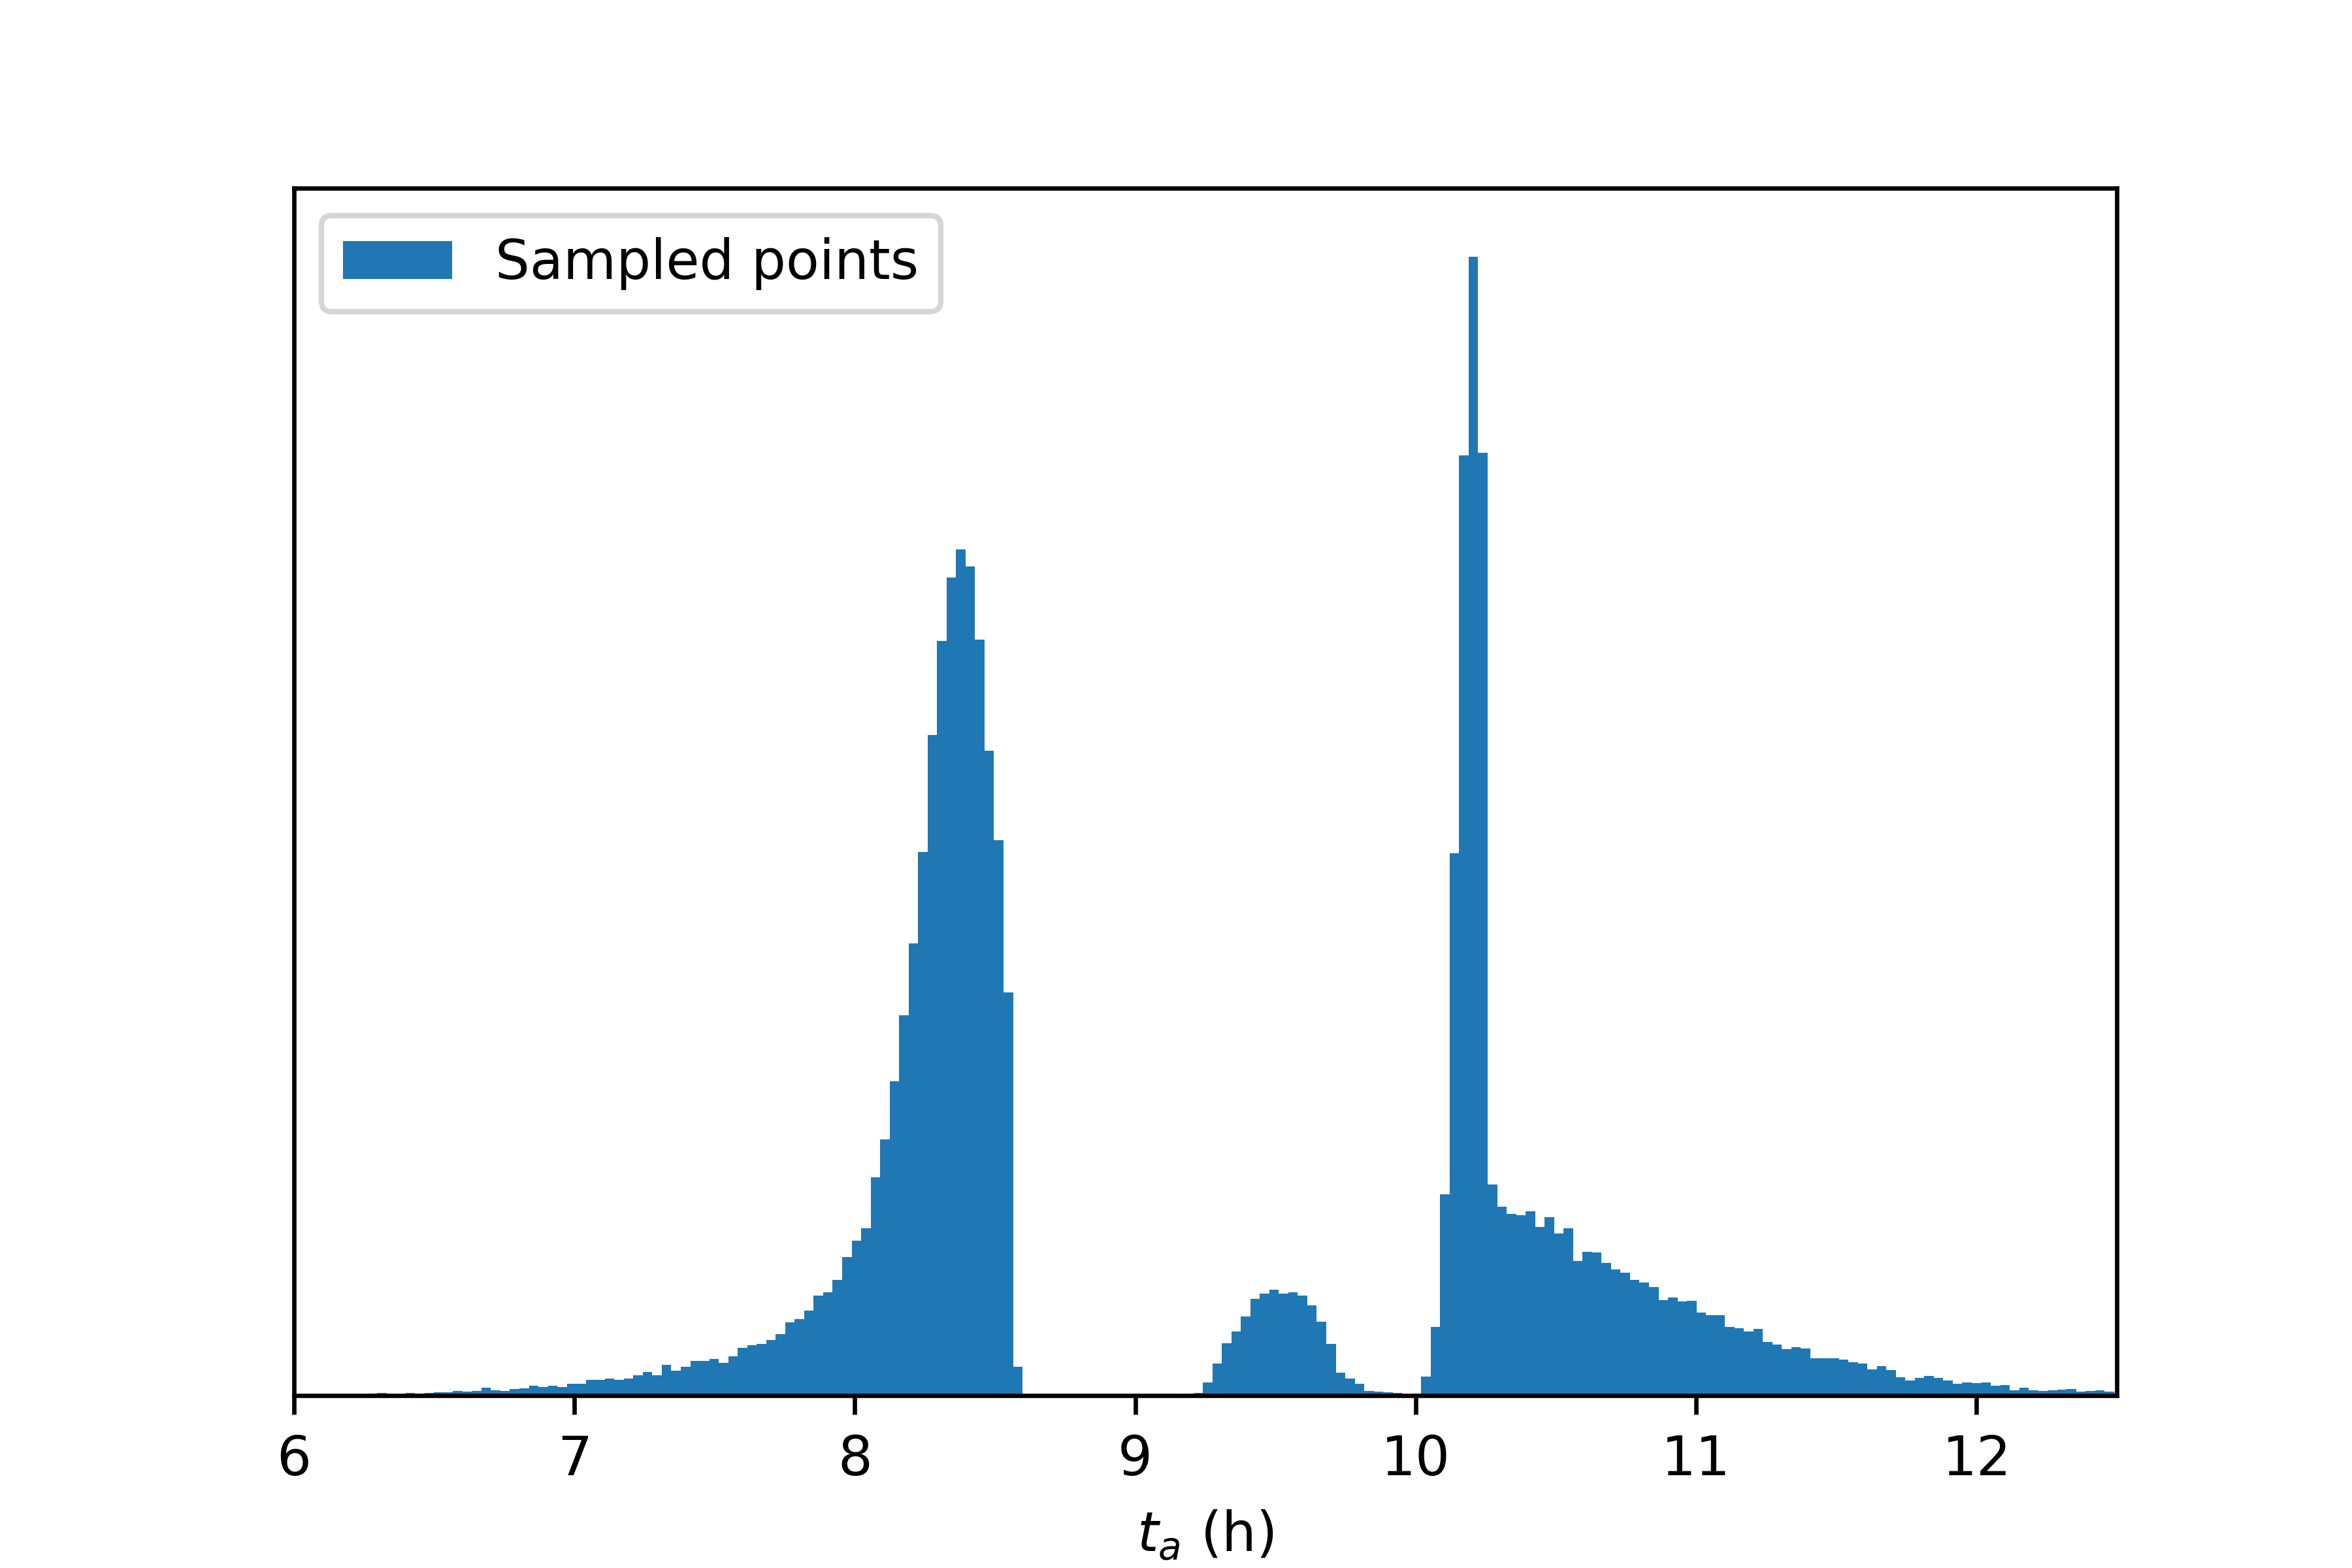
\includegraphics[width=.65\textwidth]{hist_no_ll}}{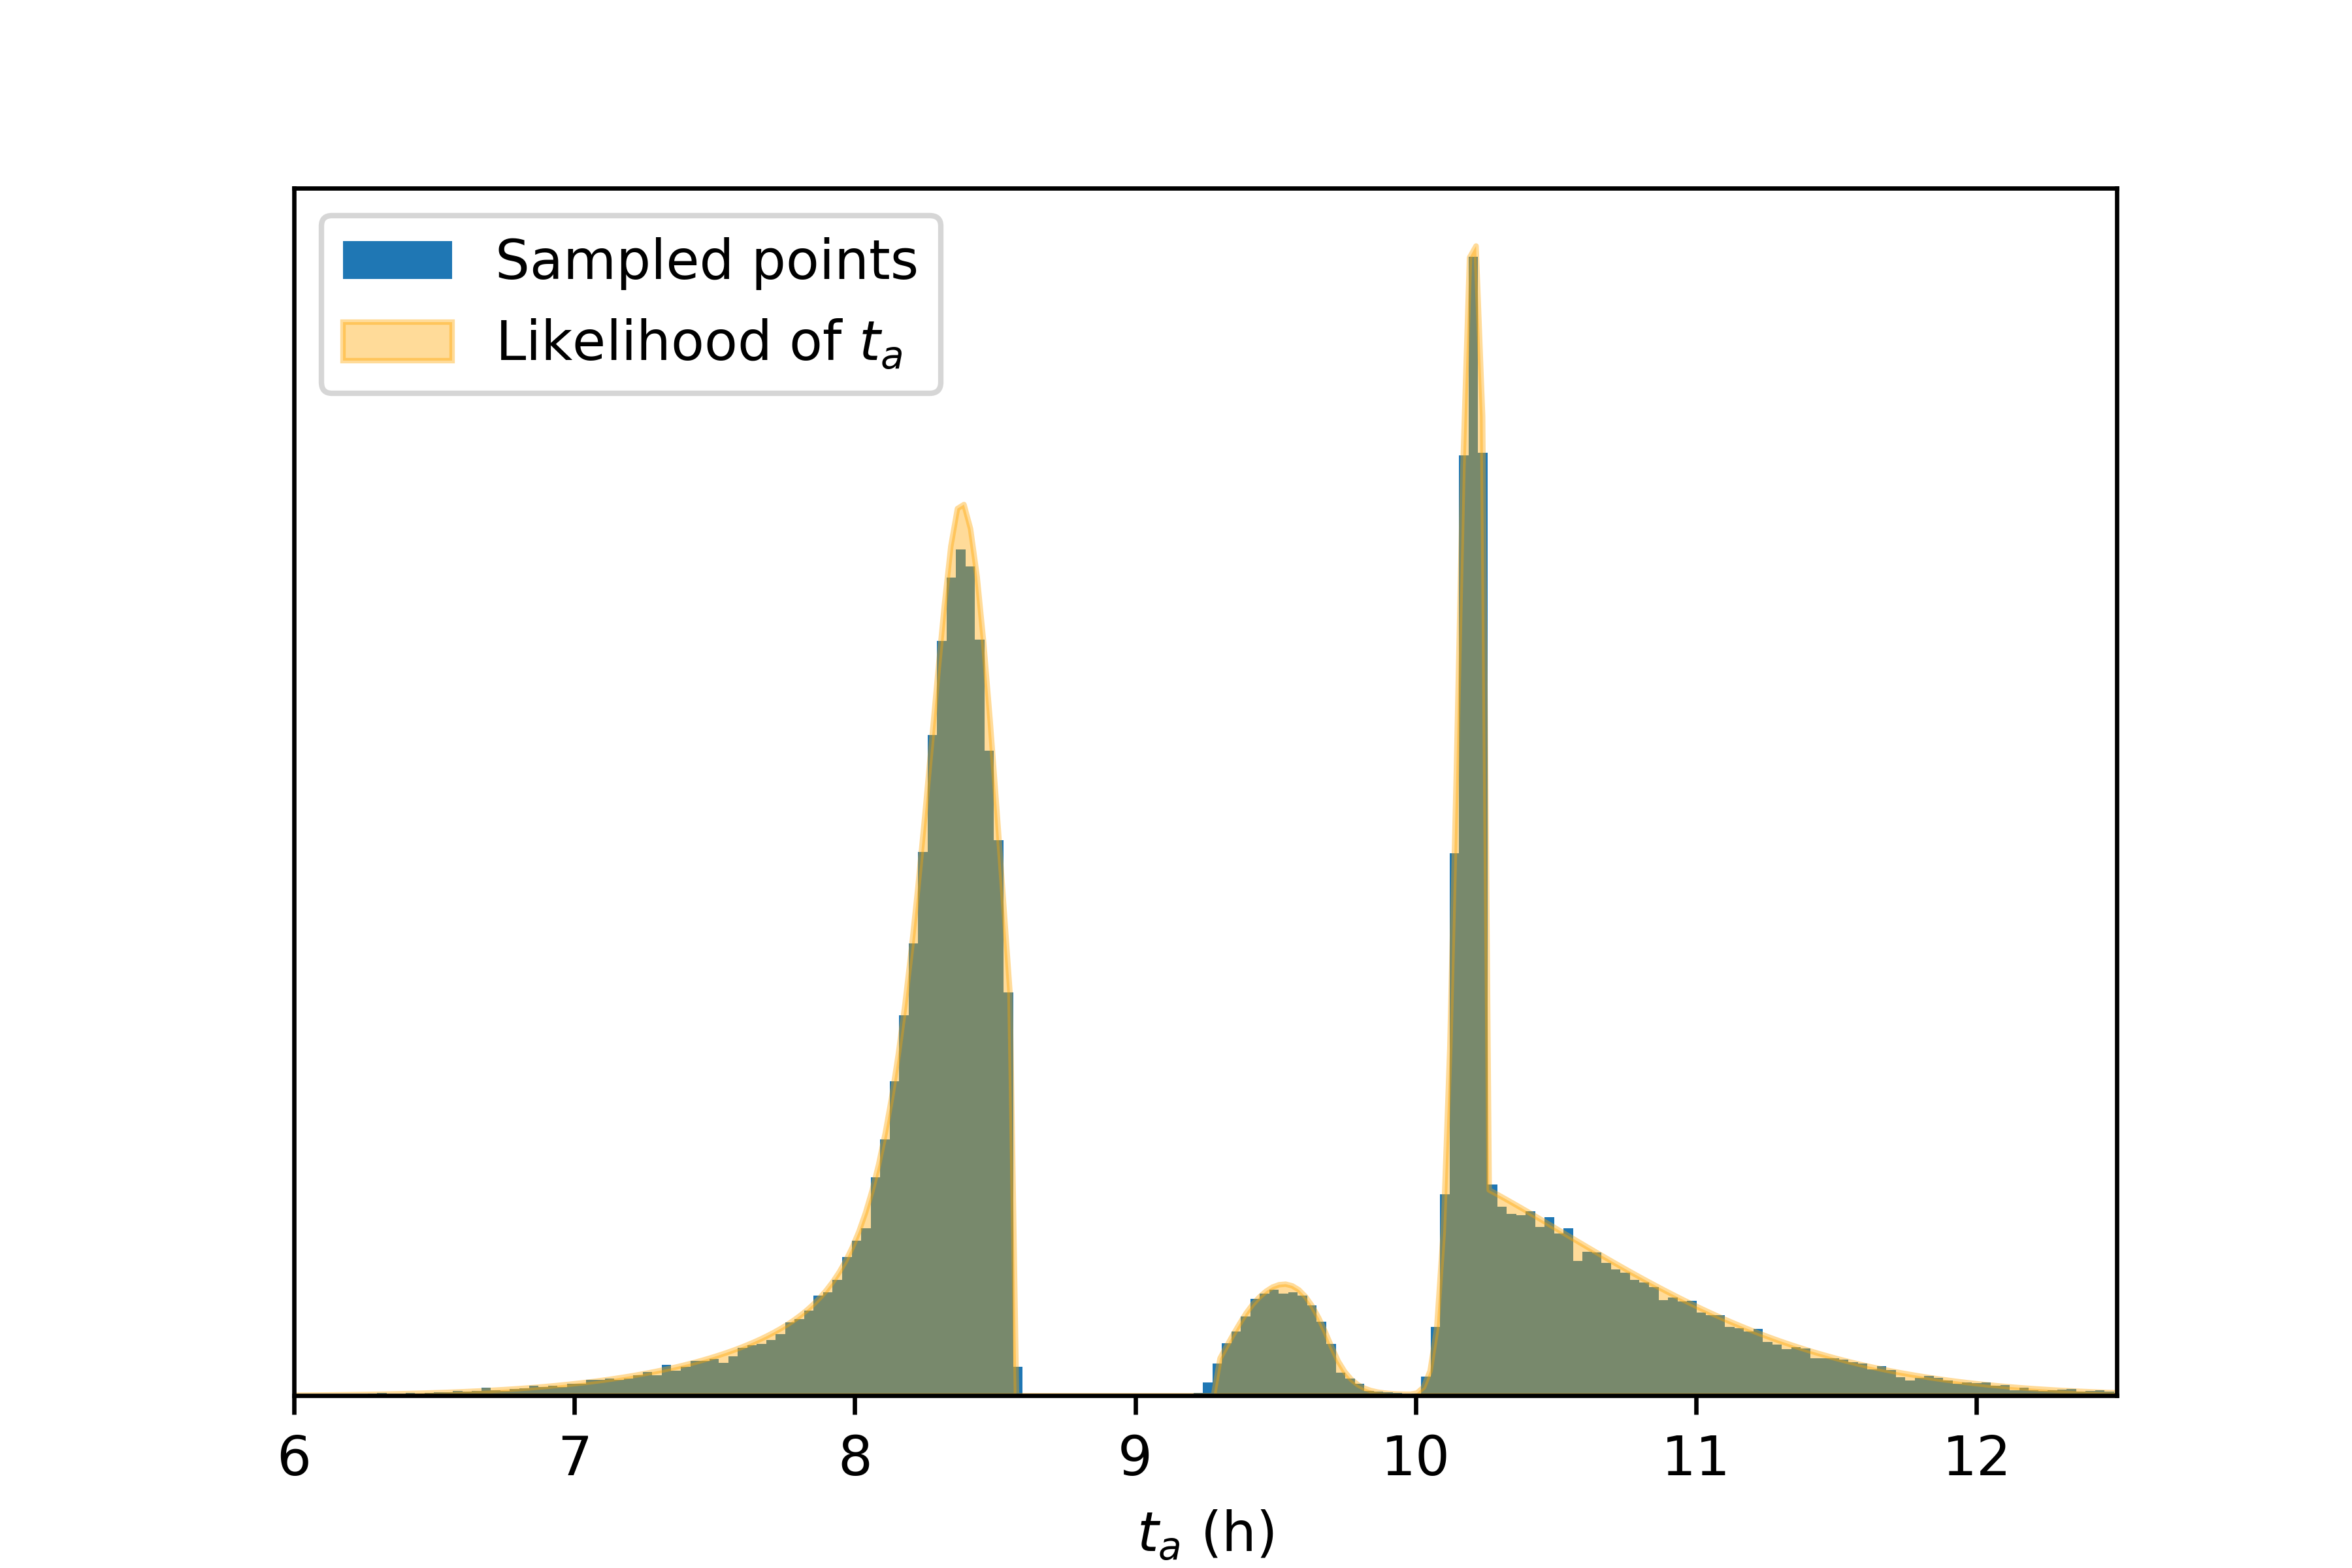
\includegraphics[width=.65\textwidth]{hist_ll}}
\end{frame}

\begin{frame}
  \frametitle{Plotting the Likelihood}
  By fixing some of the components of \(\theta\), the likelihood can be plotted when varying the rest of them.

  For \only<1>{\(\sigma = 0.3\)}\only<2>{\(\sigma = 0.03\)}\only<3>{\(\sigma = 1.3\)}

  \centering
  \only<1>{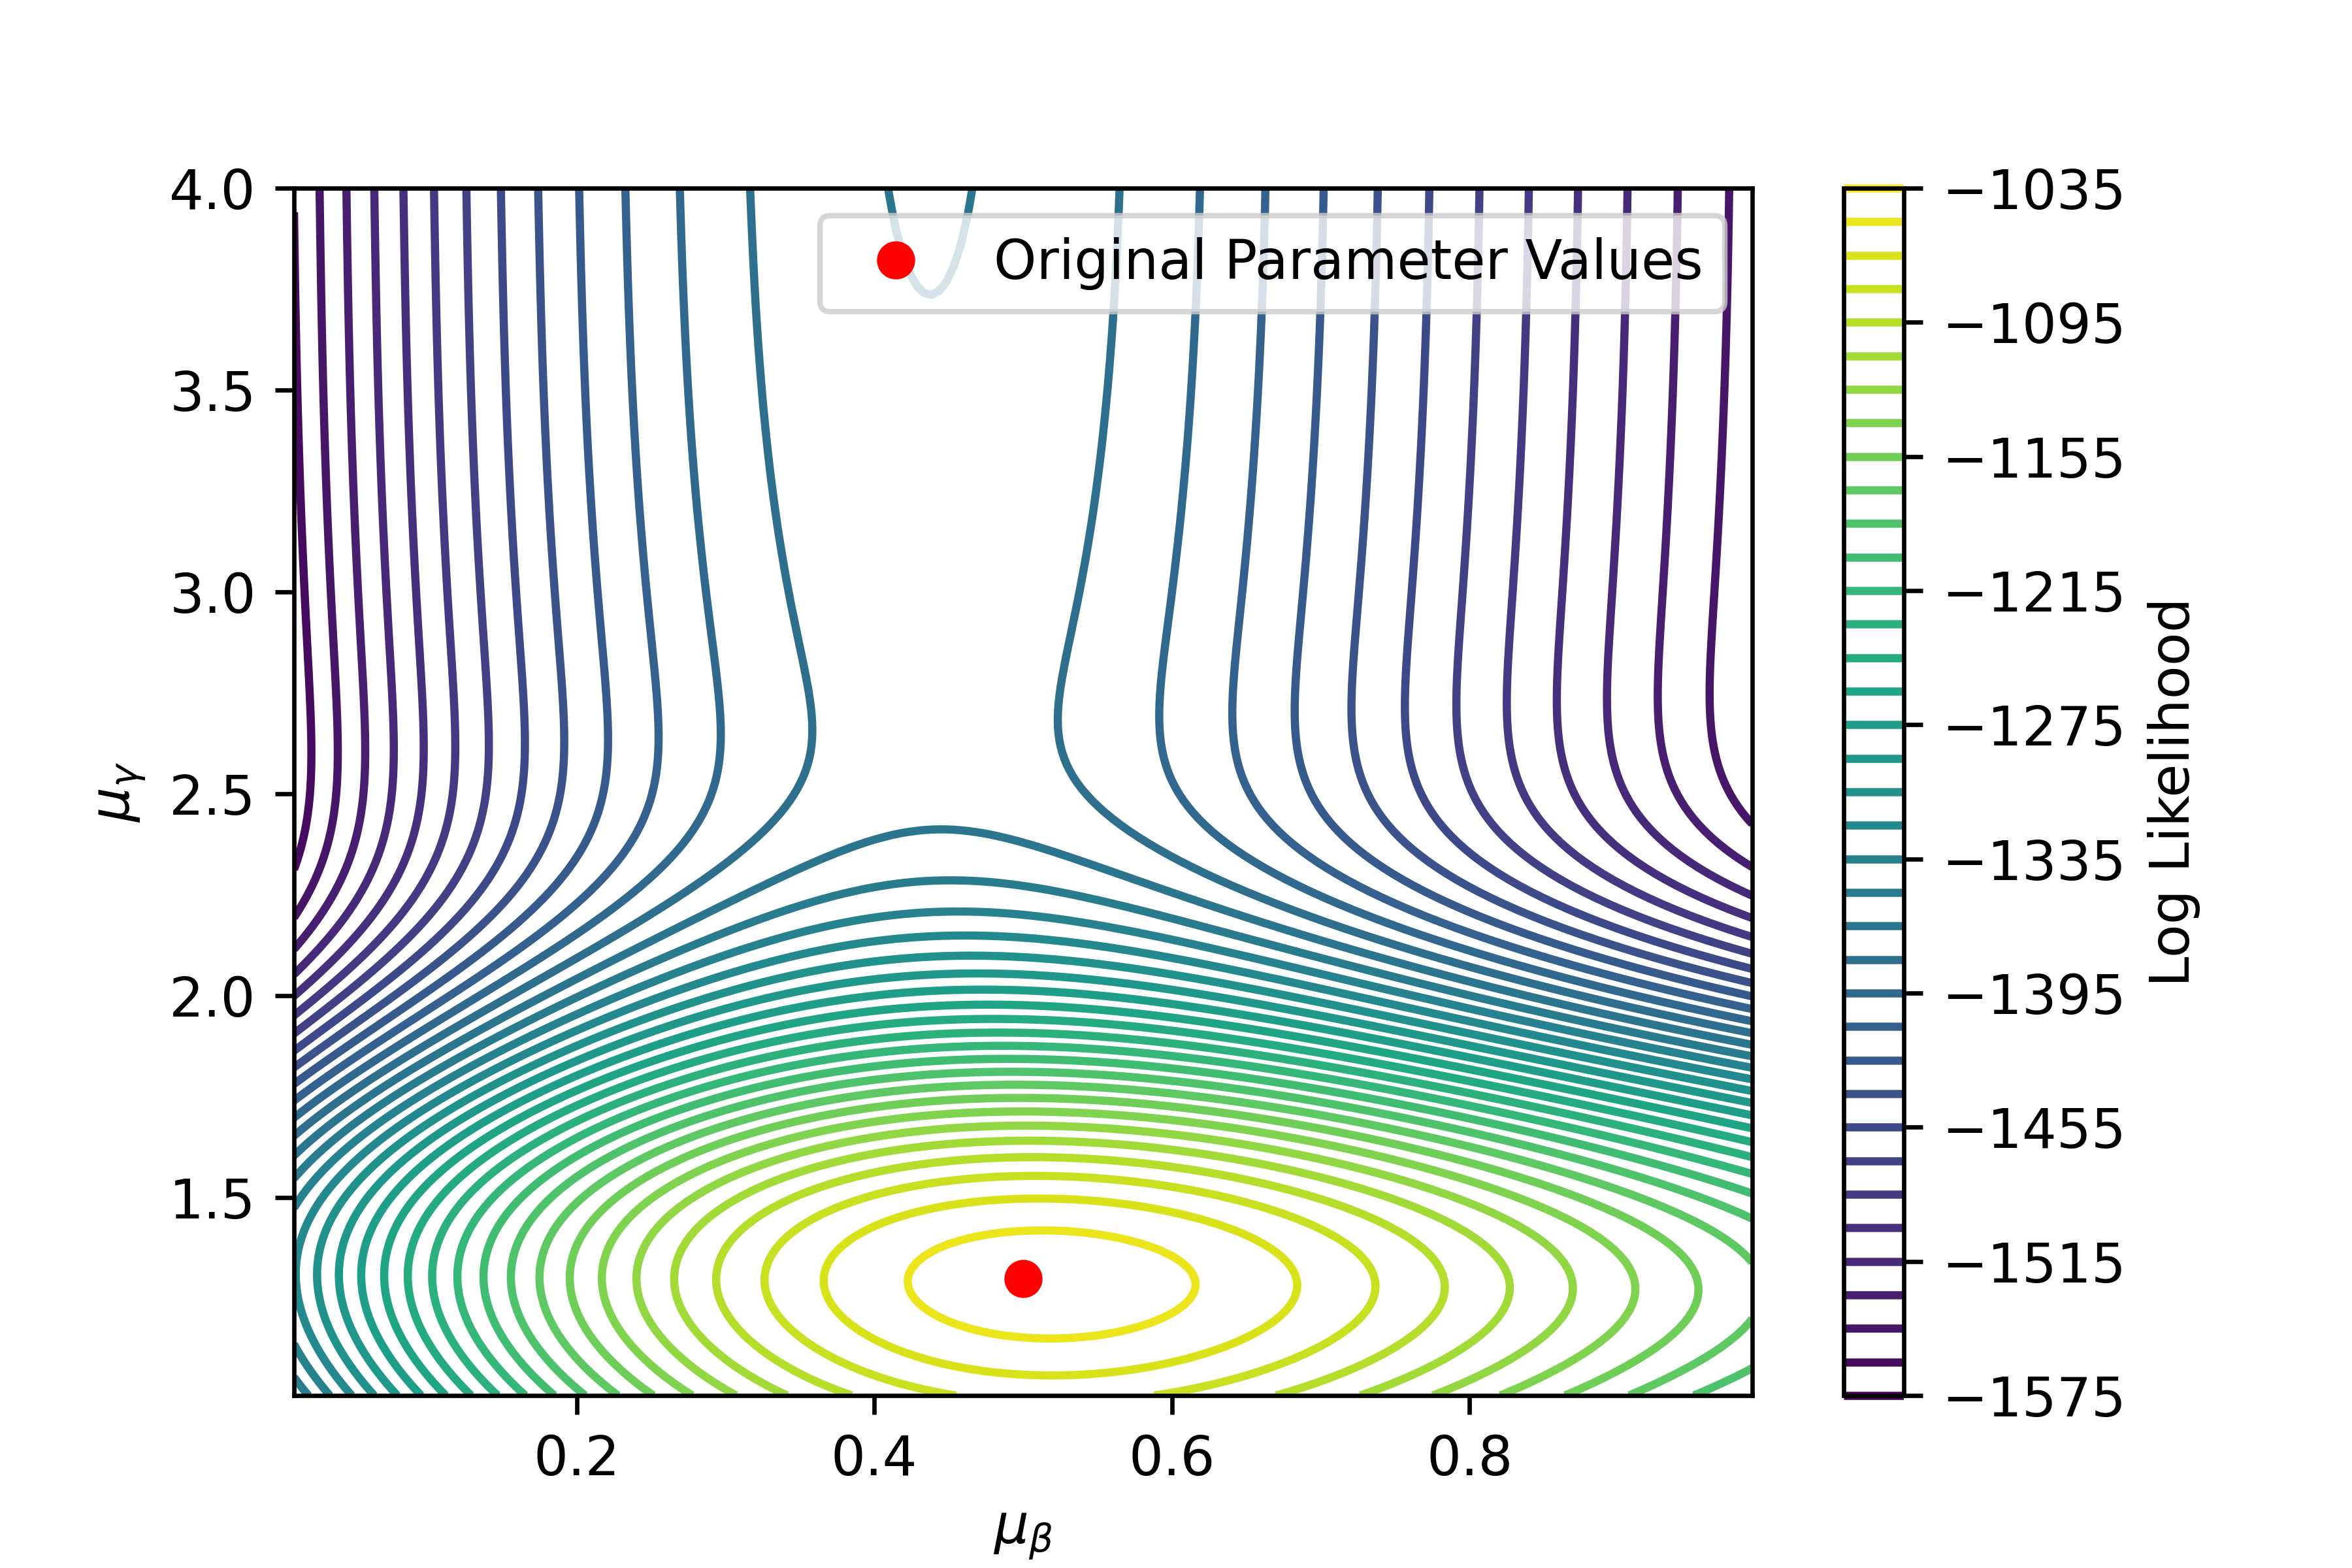
\includegraphics[width=.8\textwidth]{contour_beautiful}}
  \only<2>{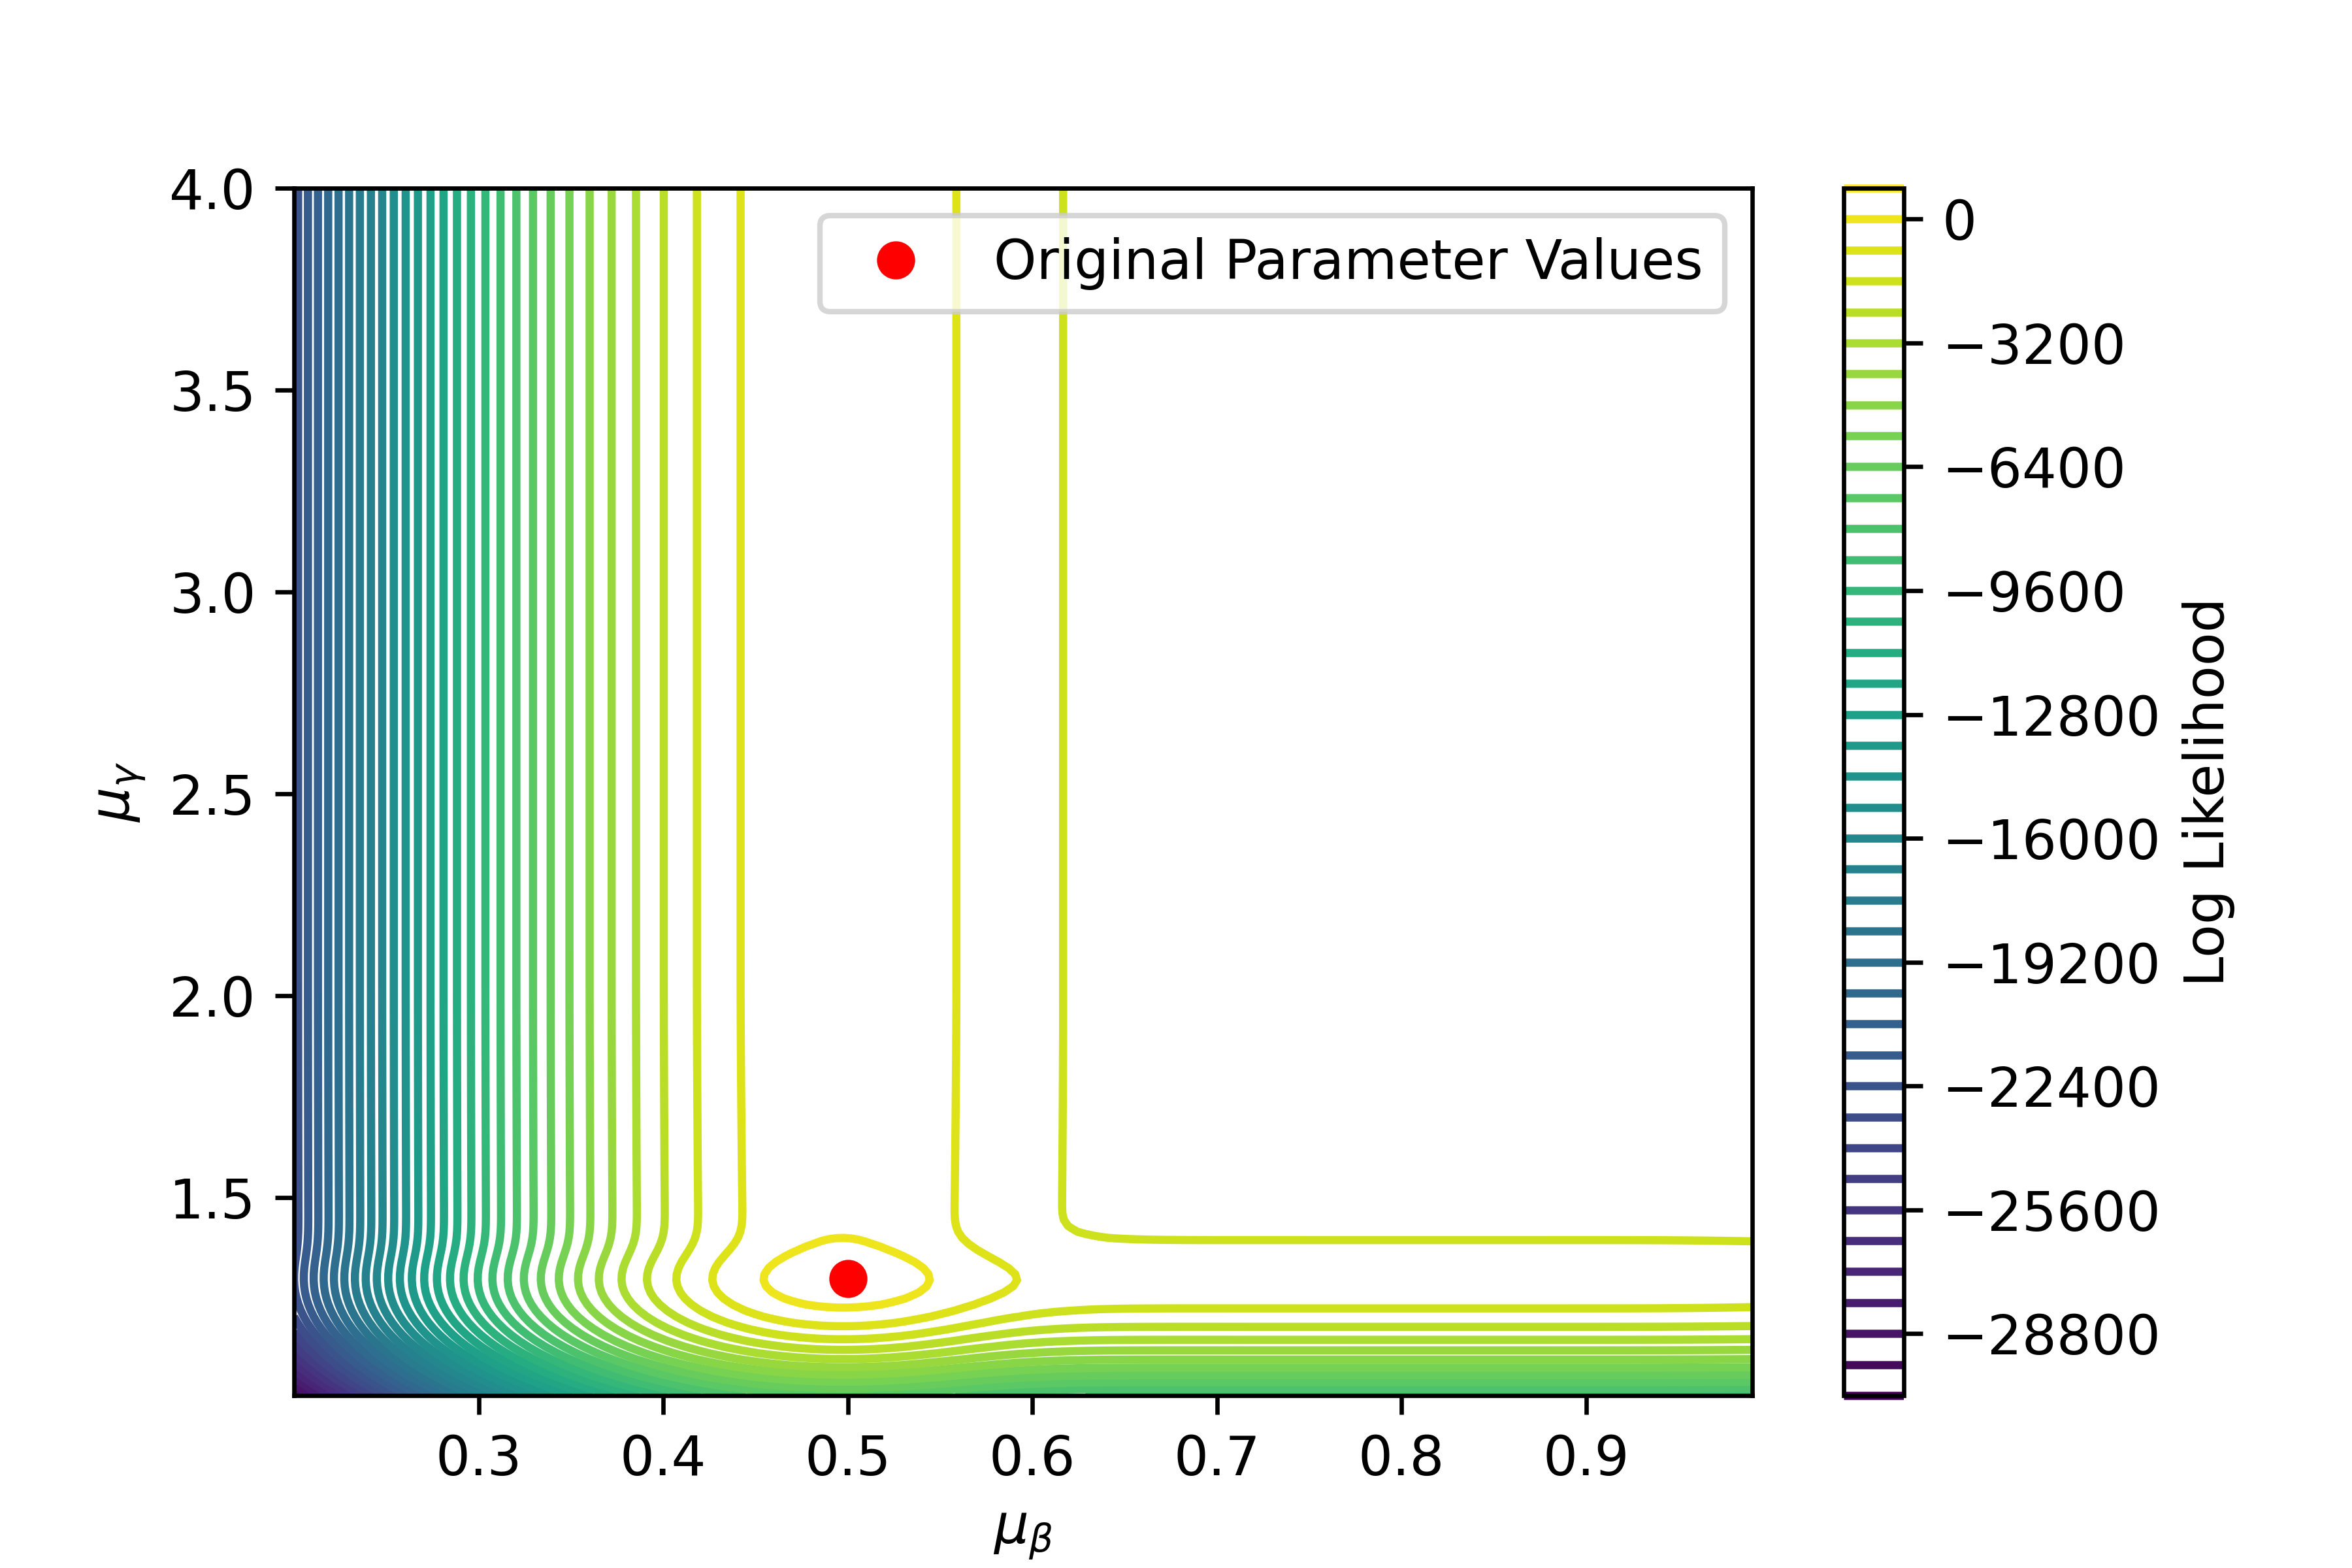
\includegraphics[width=.8\textwidth]{contour_ugly}}
  \only<3>{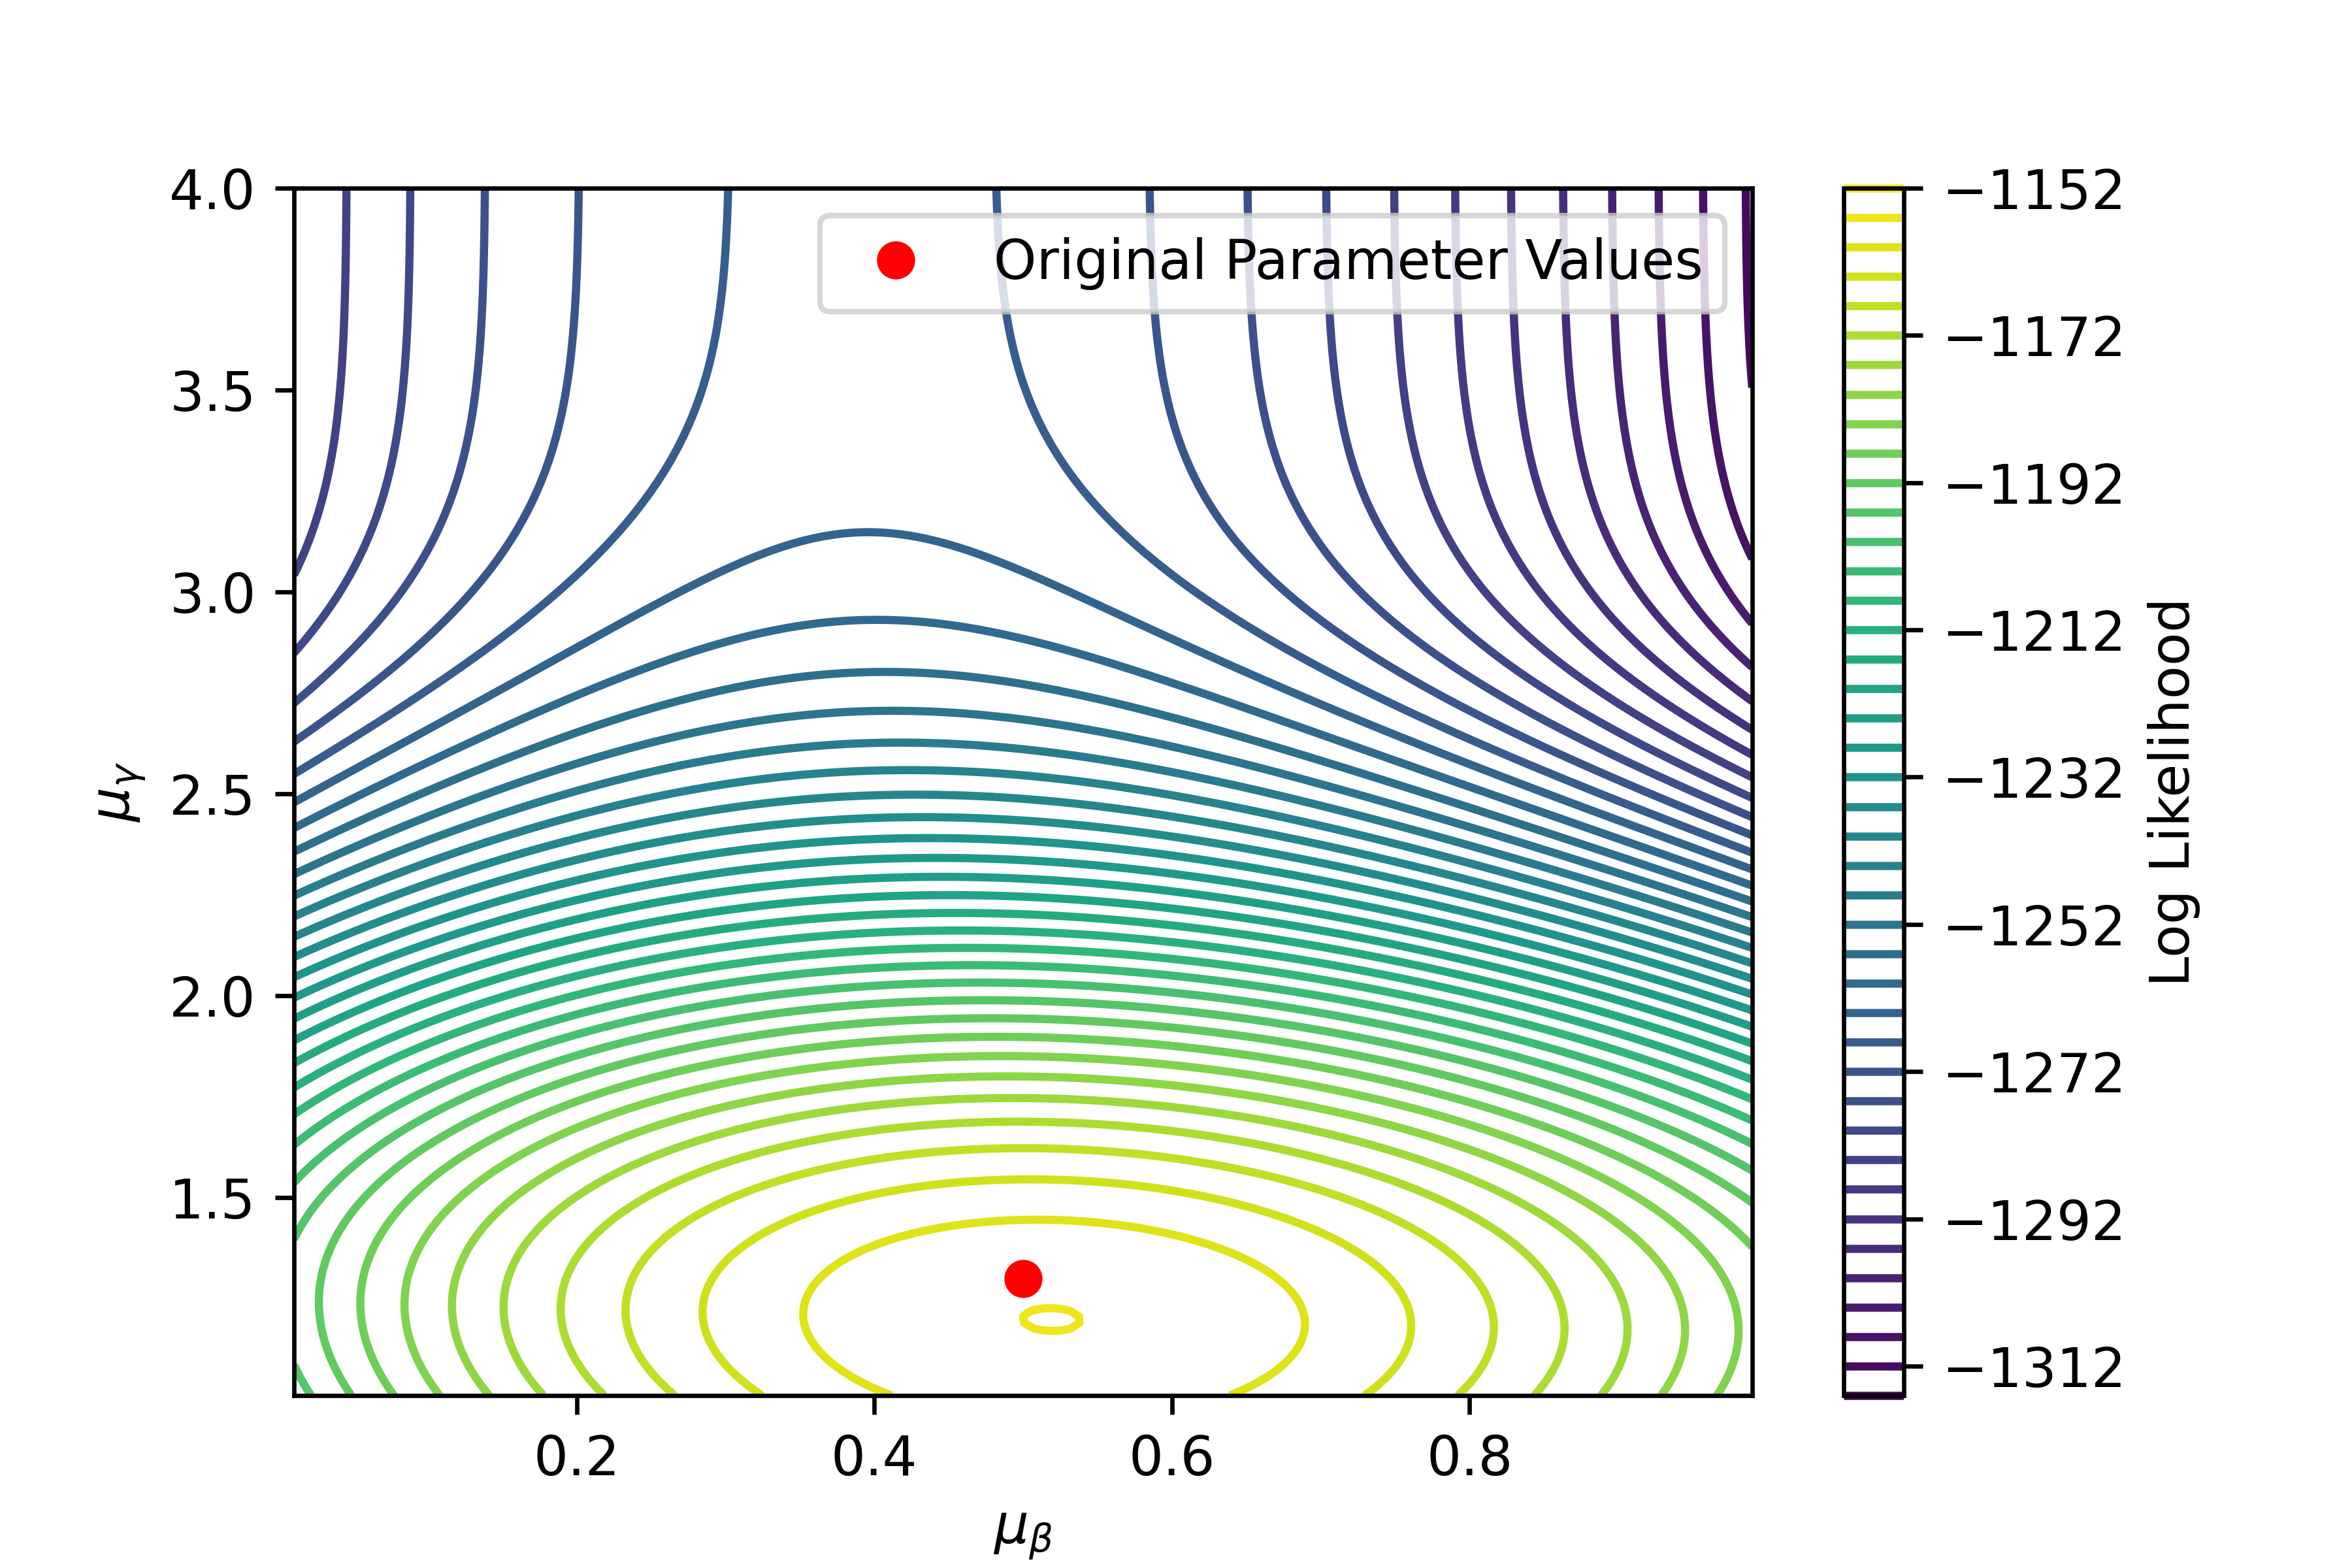
\includegraphics[width=.8\textwidth]{contour_flat}}
\end{frame}

\begin{frame}
  \frametitle{Retrieving the parameter \(\theta\)}
  Running an optimizer on the likelihood,
  the parameter \(\theta \in \mathbb{R}^5\) can be retrieved.
  \begin{itemize}
  \item<2-> Sufficient precision is achieved, even with gradient-free optimization techniques
  \item<3-> Depending on the value of the parameter \(\sigma\),
    relative error can grow as high as \(15\%\).
  \item<4-> When the variance \(\sigma\) is low, a grid search can be necessary for choosing the initial condition.
  \end{itemize}
\end{frame}

\begin{frame}
  \frametitle{Evaluation on Simulated Data}
  A framework was developed for validation on data from the traffic simulator METROPOLIS2\footcite{RePEc:ema:worpap:2024-03}.
  \begin{itemize}
  \item<2-> The simulator cannot achieve convergence without employing a logit choice model
  \item<2-> Our model assumes deterministic users
  \item<3-> Convergence cannot be achieved on data from a traffic simulator
  \end{itemize}
\end{frame}

\begin{frame}
  \frametitle{Evaluation on Real Data}
  On real data, the model shows deeper problems
  \begin{itemize}
  \item<1-> We expect the problems with simulated data to be present in real data as well
  \item<2-> \textcite{https://doi.org/10.1111/iere.12692} reveals problem with the travel time function of real data
  \end{itemize}
  \visible<3->{These problems currently prevent us from performing estimations on real data}
\end{frame}

\section{Discussion}

\begin{frame}
  \tableofcontents[currentsection]
\end{frame}

\begin{frame}
  \frametitle{Validation of the Model}
  On synthetic data, the model performs adequately.
  \begin{itemize}
  \item<2-> Good convergence shows the coherence of the developed theory
  \item<3-> Convergence on synthetic data does not validate the theory in real world
  \end{itemize}
\end{frame}

\begin{frame}
  \frametitle{Estimation on Simulated Data}
  \begin{itemize}
  \item In METROPOLIS2, arrival times are computed with a logit model.
  \item Each agent chooses its departure time according to a random variable distributed as
    \begin{equation*}
      f(t) = \frac{e^{C(t)/\mu}}{\int_0^{24} e^{C(s)/\mu} ds}
    \end{equation*}
  \item Directly estimating this random variable yields another, similar, estimation method 
  \end{itemize}
\end{frame}

\begin{frame}
  \frametitle{Extension to Real Data}
  The main purpose of the model is being deployed on real data
  \begin{itemize}
  \item<2-> As in simulated data, the problem with logit may be present
  \item<3-> Real data show as well other types of problems, as highlighted by \textcite{https://doi.org/10.1111/iere.12692}
  \end{itemize}
\end{frame}

\begin{frame}
  \frametitle{Low Slopes in Real Data}
  According to \textcite{https://doi.org/10.1111/iere.12692},
  observed slopes of the travel time function are way lower than what would be expected from equilibrium solutions
  \begin{figure}
    \centering
    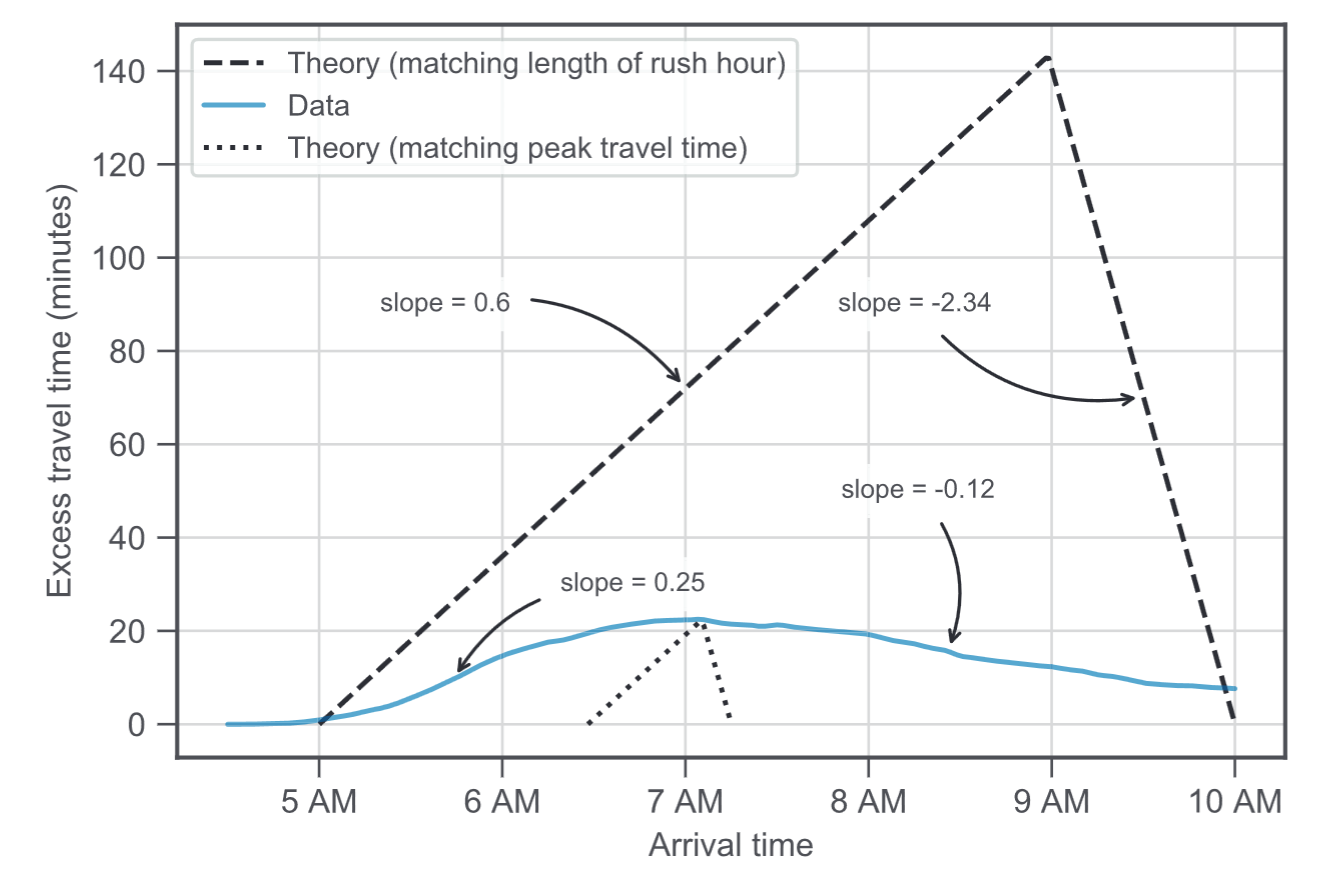
\includegraphics[width=.7\textwidth]{slopes_hall}
    \caption{Actual travel time, compared with theoretical equilibrium solution. Image taken from \textcite{https://doi.org/10.1111/iere.12692}}
  \end{figure}
\end{frame}

\begin{frame}
  \frametitle{Low slopes in Urban Data}
  \begin{itemize}
  \item The problem highlighted by \textcite{https://doi.org/10.1111/iere.12692} subsists in both urban and non-urban scenarios
  \item Our findings support it with data from 30 OD pairs in the city of Paris
  \end{itemize}
  \centering
  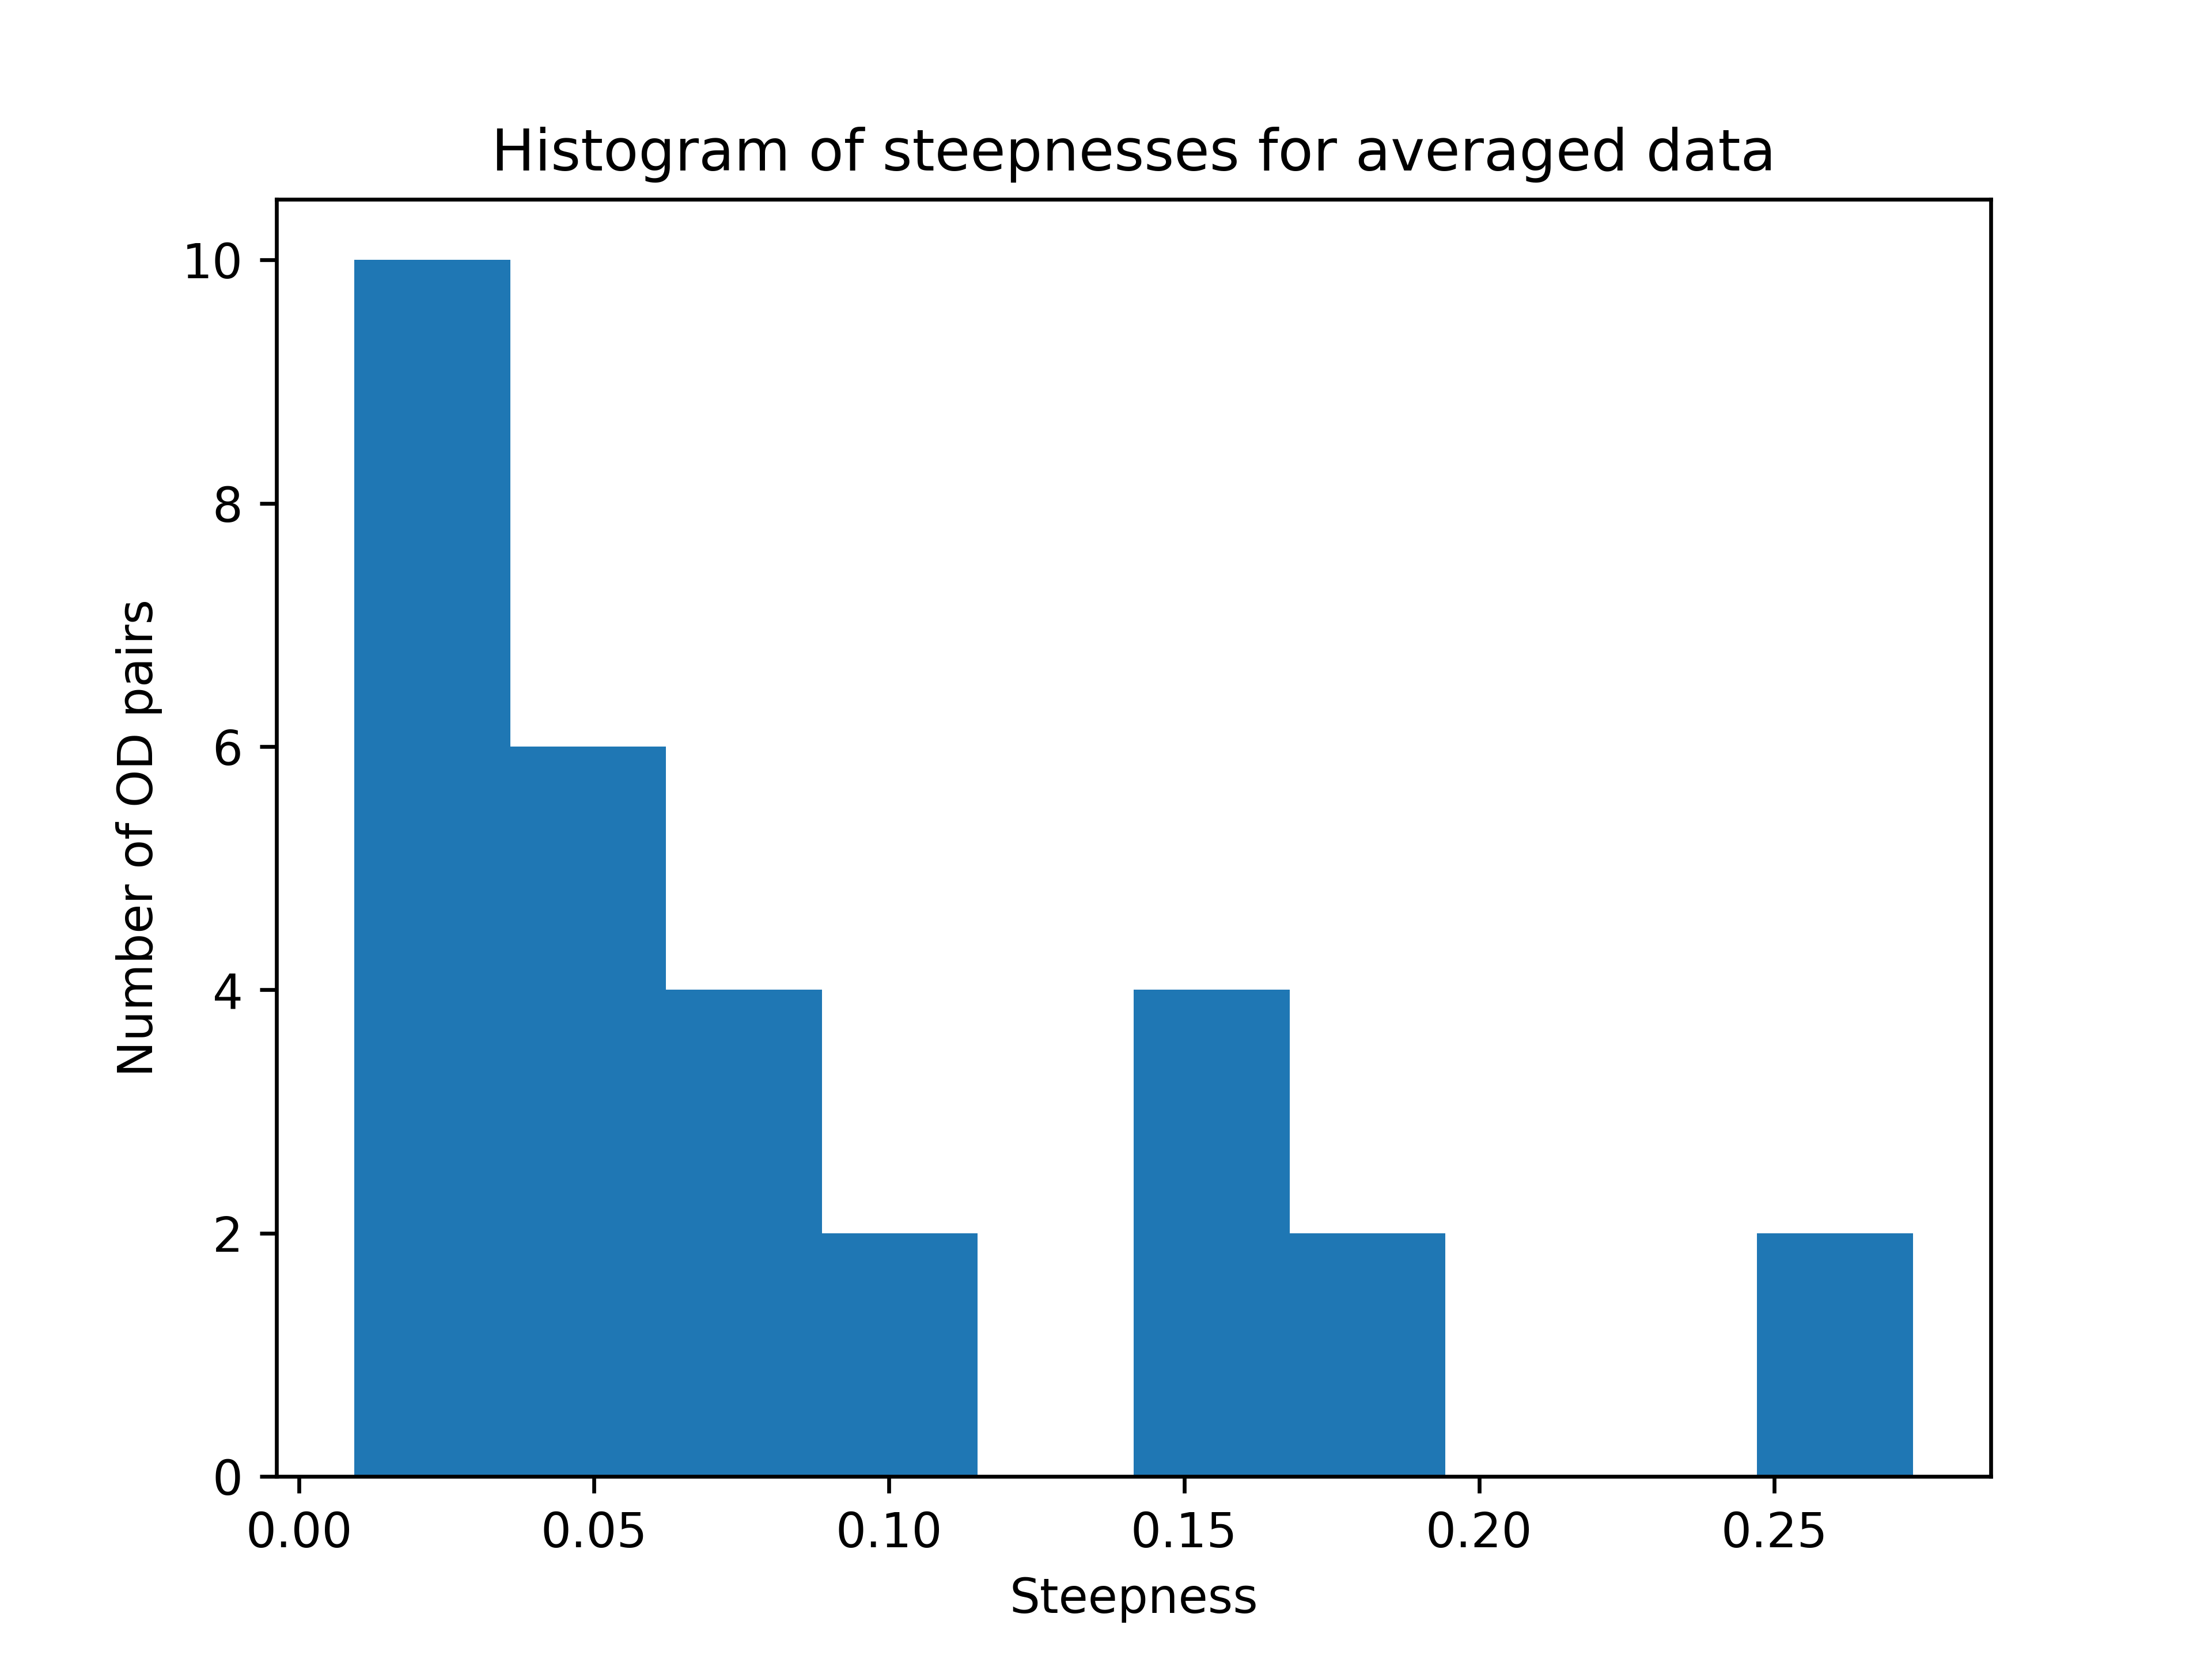
\includegraphics[width=.7\textwidth]{tomtom_hist}
\end{frame}

\begin{frame}
  \frametitle{Solving Problem about Low Slopes }
  The problem with low observable slopes can be solved in two distinct ways:
  \begin{itemize}
  \item<2-> By considering different distributions for the parameters \(\beta, \gamma\)
  \item<3-> By considering how uncertainty could affect departure times:
    perceived travel time can be considered as a stochastic process
  \end{itemize}
  \visible<4->{These methods can be subject of future research}
\end{frame}

\section{Conclusion}

\begin{frame}
  \tableofcontents[currentsection]
\end{frame}

\begin{frame}
  \frametitle{Conclusion}
  \begin{itemize}
  \item We are able to develop a model which estimates schedule delay preferences from data about observed arrivals and experienced travel time alone
  \item<2-> The model performs well on synthetic data
  \item<3-> We can't generalize on simulated data, due to the structure of the simulator
  \item<4-> On real data, deeper problems are present
  \item<5-> These problems require structural solutions, subject to future research
  \end{itemize}
\end{frame}

\begin{frame}[allowframebreaks]
  \frametitle{References}
  \printbibliography
\end{frame}

\end{document}
%%% Local Variables:
%%% mode: LaTeX
%%% TeX-master: t
%%% End:
